% Options for packages loaded elsewhere
\PassOptionsToPackage{unicode}{hyperref}
\PassOptionsToPackage{hyphens}{url}
\PassOptionsToPackage{dvipsnames,svgnames,x11names}{xcolor}
%
\documentclass[
]{book}
\usepackage{amsmath,amssymb}
\usepackage{iftex}
\ifPDFTeX
  \usepackage[T1]{fontenc}
  \usepackage[utf8]{inputenc}
  \usepackage{textcomp} % provide euro and other symbols
\else % if luatex or xetex
  \usepackage{unicode-math} % this also loads fontspec
  \defaultfontfeatures{Scale=MatchLowercase}
  \defaultfontfeatures[\rmfamily]{Ligatures=TeX,Scale=1}
\fi
\usepackage{lmodern}
\ifPDFTeX\else
  % xetex/luatex font selection
\fi
% Use upquote if available, for straight quotes in verbatim environments
\IfFileExists{upquote.sty}{\usepackage{upquote}}{}
\IfFileExists{microtype.sty}{% use microtype if available
  \usepackage[]{microtype}
  \UseMicrotypeSet[protrusion]{basicmath} % disable protrusion for tt fonts
}{}
\makeatletter
\@ifundefined{KOMAClassName}{% if non-KOMA class
  \IfFileExists{parskip.sty}{%
    \usepackage{parskip}
  }{% else
    \setlength{\parindent}{0pt}
    \setlength{\parskip}{6pt plus 2pt minus 1pt}}
}{% if KOMA class
  \KOMAoptions{parskip=half}}
\makeatother
\usepackage{xcolor}
\usepackage{color}
\usepackage{fancyvrb}
\newcommand{\VerbBar}{|}
\newcommand{\VERB}{\Verb[commandchars=\\\{\}]}
\DefineVerbatimEnvironment{Highlighting}{Verbatim}{commandchars=\\\{\}}
% Add ',fontsize=\small' for more characters per line
\usepackage{framed}
\definecolor{shadecolor}{RGB}{248,248,248}
\newenvironment{Shaded}{\begin{snugshade}}{\end{snugshade}}
\newcommand{\AlertTok}[1]{\textcolor[rgb]{0.94,0.16,0.16}{#1}}
\newcommand{\AnnotationTok}[1]{\textcolor[rgb]{0.56,0.35,0.01}{\textbf{\textit{#1}}}}
\newcommand{\AttributeTok}[1]{\textcolor[rgb]{0.13,0.29,0.53}{#1}}
\newcommand{\BaseNTok}[1]{\textcolor[rgb]{0.00,0.00,0.81}{#1}}
\newcommand{\BuiltInTok}[1]{#1}
\newcommand{\CharTok}[1]{\textcolor[rgb]{0.31,0.60,0.02}{#1}}
\newcommand{\CommentTok}[1]{\textcolor[rgb]{0.56,0.35,0.01}{\textit{#1}}}
\newcommand{\CommentVarTok}[1]{\textcolor[rgb]{0.56,0.35,0.01}{\textbf{\textit{#1}}}}
\newcommand{\ConstantTok}[1]{\textcolor[rgb]{0.56,0.35,0.01}{#1}}
\newcommand{\ControlFlowTok}[1]{\textcolor[rgb]{0.13,0.29,0.53}{\textbf{#1}}}
\newcommand{\DataTypeTok}[1]{\textcolor[rgb]{0.13,0.29,0.53}{#1}}
\newcommand{\DecValTok}[1]{\textcolor[rgb]{0.00,0.00,0.81}{#1}}
\newcommand{\DocumentationTok}[1]{\textcolor[rgb]{0.56,0.35,0.01}{\textbf{\textit{#1}}}}
\newcommand{\ErrorTok}[1]{\textcolor[rgb]{0.64,0.00,0.00}{\textbf{#1}}}
\newcommand{\ExtensionTok}[1]{#1}
\newcommand{\FloatTok}[1]{\textcolor[rgb]{0.00,0.00,0.81}{#1}}
\newcommand{\FunctionTok}[1]{\textcolor[rgb]{0.13,0.29,0.53}{\textbf{#1}}}
\newcommand{\ImportTok}[1]{#1}
\newcommand{\InformationTok}[1]{\textcolor[rgb]{0.56,0.35,0.01}{\textbf{\textit{#1}}}}
\newcommand{\KeywordTok}[1]{\textcolor[rgb]{0.13,0.29,0.53}{\textbf{#1}}}
\newcommand{\NormalTok}[1]{#1}
\newcommand{\OperatorTok}[1]{\textcolor[rgb]{0.81,0.36,0.00}{\textbf{#1}}}
\newcommand{\OtherTok}[1]{\textcolor[rgb]{0.56,0.35,0.01}{#1}}
\newcommand{\PreprocessorTok}[1]{\textcolor[rgb]{0.56,0.35,0.01}{\textit{#1}}}
\newcommand{\RegionMarkerTok}[1]{#1}
\newcommand{\SpecialCharTok}[1]{\textcolor[rgb]{0.81,0.36,0.00}{\textbf{#1}}}
\newcommand{\SpecialStringTok}[1]{\textcolor[rgb]{0.31,0.60,0.02}{#1}}
\newcommand{\StringTok}[1]{\textcolor[rgb]{0.31,0.60,0.02}{#1}}
\newcommand{\VariableTok}[1]{\textcolor[rgb]{0.00,0.00,0.00}{#1}}
\newcommand{\VerbatimStringTok}[1]{\textcolor[rgb]{0.31,0.60,0.02}{#1}}
\newcommand{\WarningTok}[1]{\textcolor[rgb]{0.56,0.35,0.01}{\textbf{\textit{#1}}}}
\usepackage{longtable,booktabs,array}
\usepackage{calc} % for calculating minipage widths
% Correct order of tables after \paragraph or \subparagraph
\usepackage{etoolbox}
\makeatletter
\patchcmd\longtable{\par}{\if@noskipsec\mbox{}\fi\par}{}{}
\makeatother
% Allow footnotes in longtable head/foot
\IfFileExists{footnotehyper.sty}{\usepackage{footnotehyper}}{\usepackage{footnote}}
\makesavenoteenv{longtable}
\usepackage{graphicx}
\makeatletter
\def\maxwidth{\ifdim\Gin@nat@width>\linewidth\linewidth\else\Gin@nat@width\fi}
\def\maxheight{\ifdim\Gin@nat@height>\textheight\textheight\else\Gin@nat@height\fi}
\makeatother
% Scale images if necessary, so that they will not overflow the page
% margins by default, and it is still possible to overwrite the defaults
% using explicit options in \includegraphics[width, height, ...]{}
\setkeys{Gin}{width=\maxwidth,height=\maxheight,keepaspectratio}
% Set default figure placement to htbp
\makeatletter
\def\fps@figure{htbp}
\makeatother
\setlength{\emergencystretch}{3em} % prevent overfull lines
\providecommand{\tightlist}{%
  \setlength{\itemsep}{0pt}\setlength{\parskip}{0pt}}
\setcounter{secnumdepth}{5}
\usepackage{booktabs}
\ifLuaTeX
  \usepackage{selnolig}  % disable illegal ligatures
\fi
\usepackage[]{natbib}
\bibliographystyle{plainnat}
\IfFileExists{bookmark.sty}{\usepackage{bookmark}}{\usepackage{hyperref}}
\IfFileExists{xurl.sty}{\usepackage{xurl}}{} % add URL line breaks if available
\urlstyle{same}
\hypersetup{
  pdftitle={An introduction R},
  pdfauthor={Saneesh},
  colorlinks=true,
  linkcolor={Maroon},
  filecolor={Maroon},
  citecolor={Blue},
  urlcolor={blue},
  pdfcreator={LaTeX via pandoc}}

\title{An introduction R}
\author{Saneesh}
\date{2024-03-01}

\begin{document}
\maketitle

{
\hypersetup{linkcolor=}
\setcounter{tocdepth}{1}
\tableofcontents
}
\hypertarget{about}{%
\chapter{About}\label{about}}

This is book is an introduction to R using \texttt{tidyverse} packages (Figure 1.1) and wrote using the \texttt{bookdown} package.

\begin{figure}

{\centering 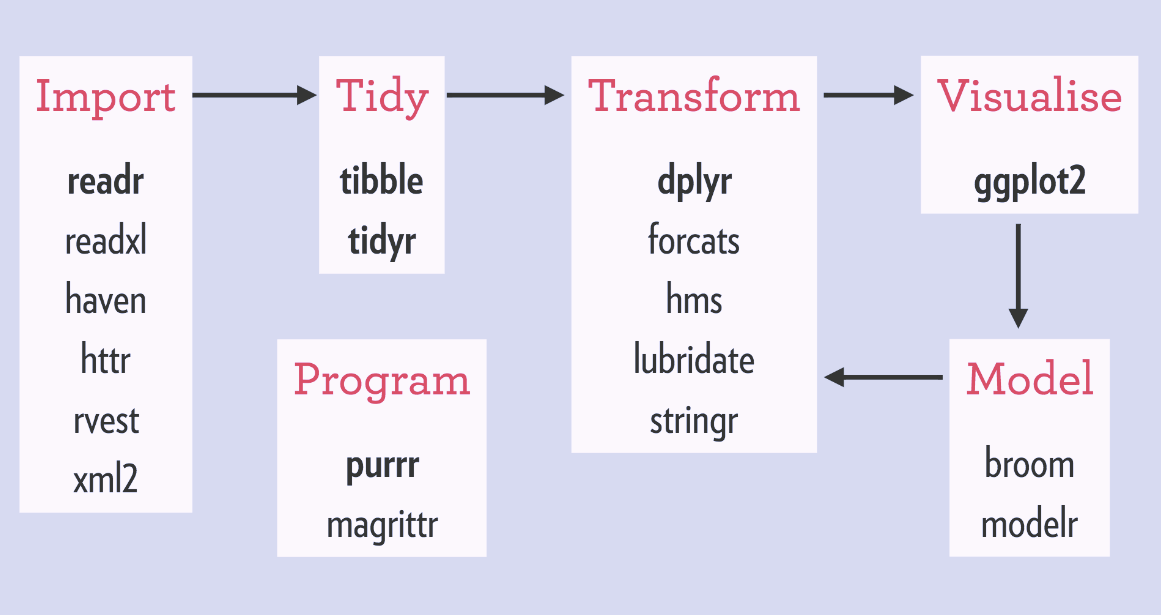
\includegraphics[width=0.7\linewidth]{pictures/tidyverse-overview} 

}

\caption{Tidyverse packages}\label{fig:unnamed-chunk-1}
\end{figure}

\hypertarget{how-to-use-this-book}{%
\section{How to use this book}\label{how-to-use-this-book}}

Any text see inside the \texttt{grey} box is a \texttt{code}, you can copy that and paste in your \texttt{R} script.

\begin{Shaded}
\begin{Highlighting}[]
\FunctionTok{sum}\NormalTok{(}\DecValTok{1}\SpecialCharTok{+}\DecValTok{2}\NormalTok{)}
\end{Highlighting}
\end{Shaded}

\begin{verbatim}
## [1] 3
\end{verbatim}

Any text or line starts with \texttt{\#\#\ {[}1{]}\ 3} is an output of the code.

\hypertarget{installation}{%
\section{Installation}\label{installation}}

Download and install \texttt{R}. Follow the link below and choose the appropriate version.

Link: \href{https://cran.r-project.org/bin/windows/base/}{R-Windows}\\
Link: \href{https://cran.r-project.org/bin/macosx/}{R-Mac}\\
Link: \href{https://cran.r-project.org/bin/linux/ubuntu/fullREADME.html}{R-Ubuntu}\\
Download and install \texttt{RStudio}. \texttt{RStudio} is an interface which facilitates coding in \texttt{R}. We recommend \texttt{RStudio} Desktop.

Link: \href{https://posit.co/download/rstudio-desktop/}{RStudio}

\hypertarget{project}{%
\section{Project}\label{project}}

RStudio projects make it straightforward to divide your work into multiple contexts, each with their own working directory, workspace, history, and source documents.
1. Make a \texttt{New\ Folder}

\begin{figure}

{\centering 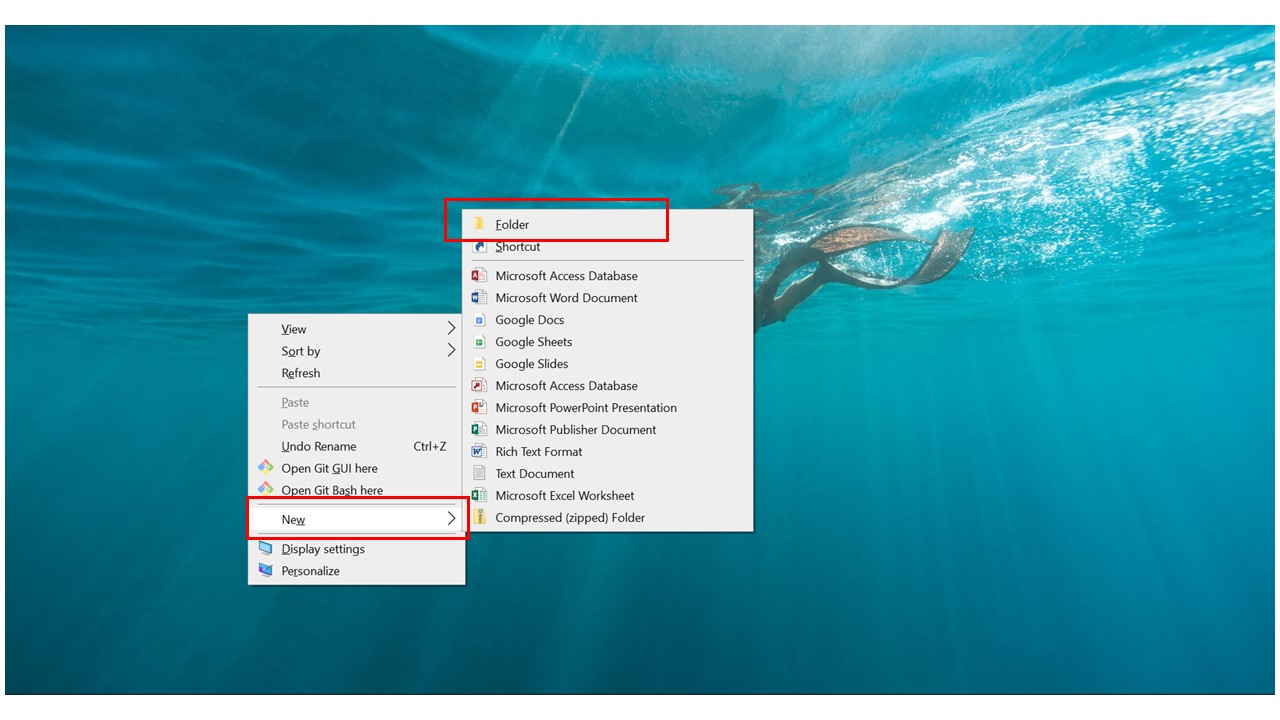
\includegraphics[width=0.7\linewidth]{pictures/Slide5} 

}

\caption{New Folder}\label{fig:unnamed-chunk-3}
\end{figure}

E.g, I made a folder \texttt{TISS\_R}

\begin{figure}

{\centering 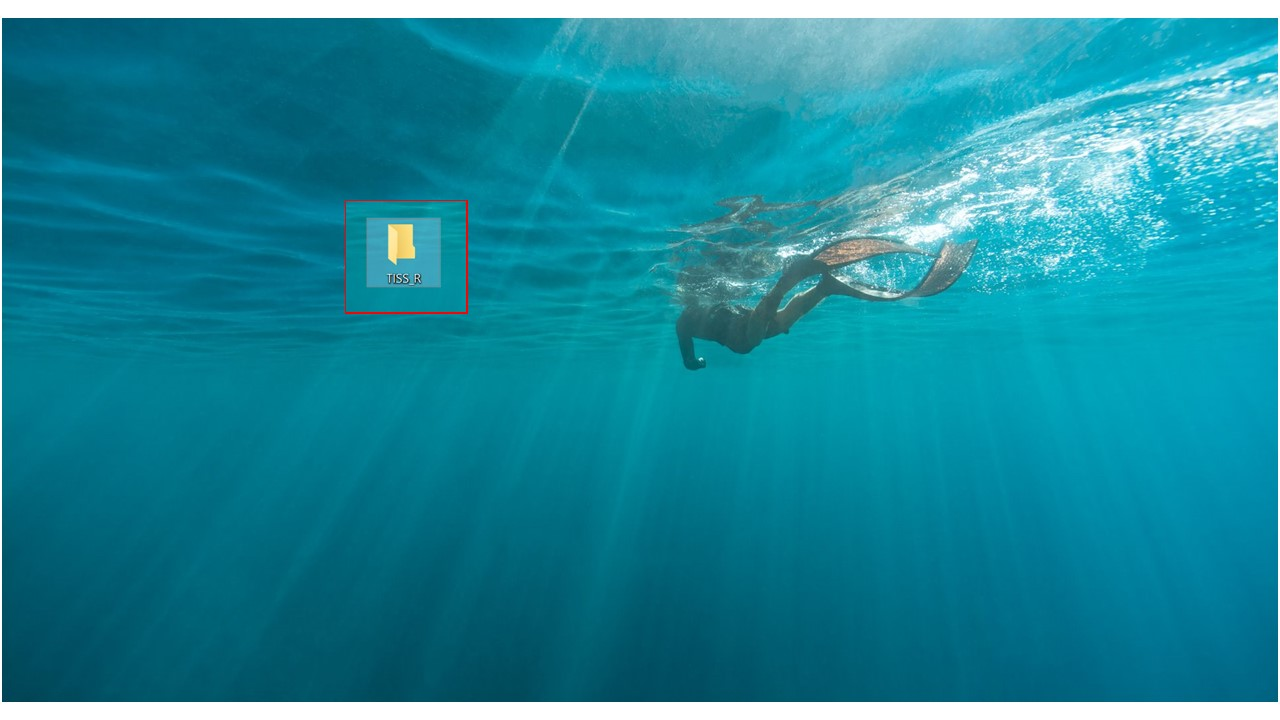
\includegraphics[width=0.7\linewidth]{pictures/Slide6} 

}

\caption{New Folder}\label{fig:unnamed-chunk-4}
\end{figure}

\begin{enumerate}
\def\labelenumi{\arabic{enumi}.}
\setcounter{enumi}{1}
\tightlist
\item
  Open \texttt{RStudio} and start a \texttt{New\ Project}
\end{enumerate}

\begin{figure}

{\centering 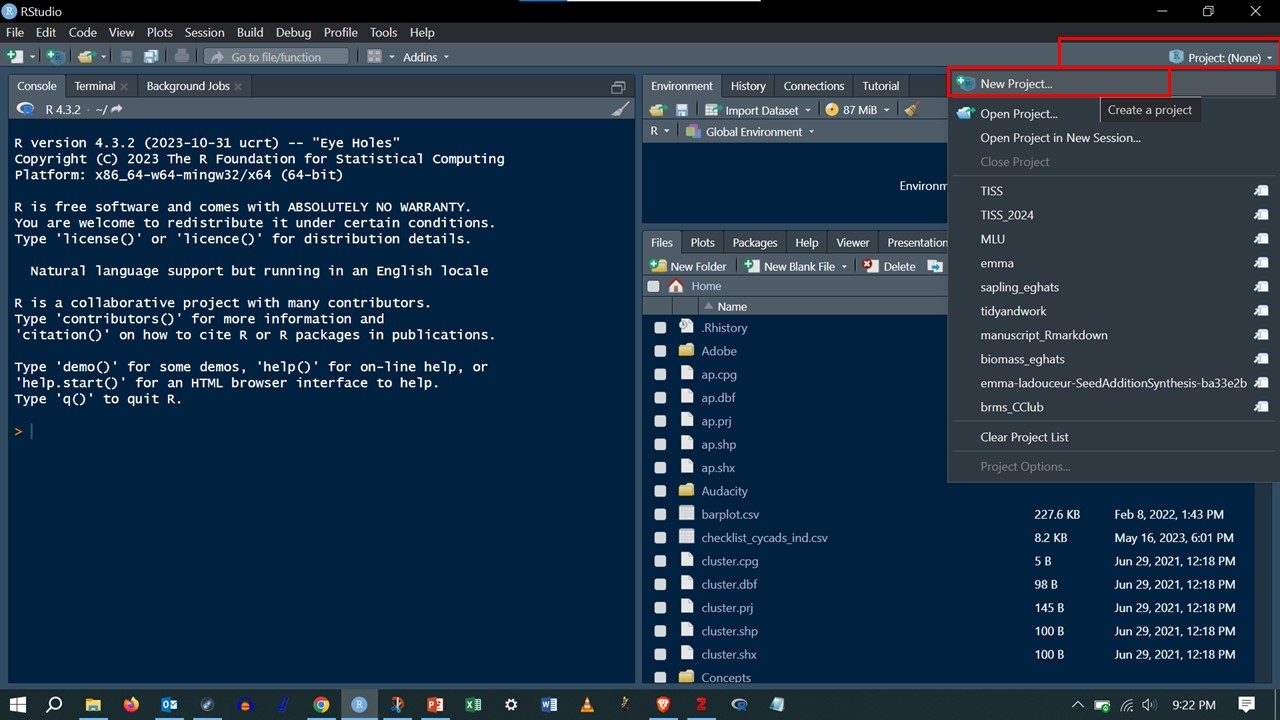
\includegraphics[width=0.7\linewidth]{pictures/Slide7} 

}

\caption{New Project}\label{fig:unnamed-chunk-5}
\end{figure}

Or from \texttt{File} \textgreater{} \texttt{New\ Project}
Because we have a folder made with name \texttt{TISS\_R} I am going to select \texttt{Existing\ Directory} if you don't have a folder select \texttt{New\ Directory} and select a location. The name of the directory or the folder will be the new project's name.

\begin{figure}

{\centering 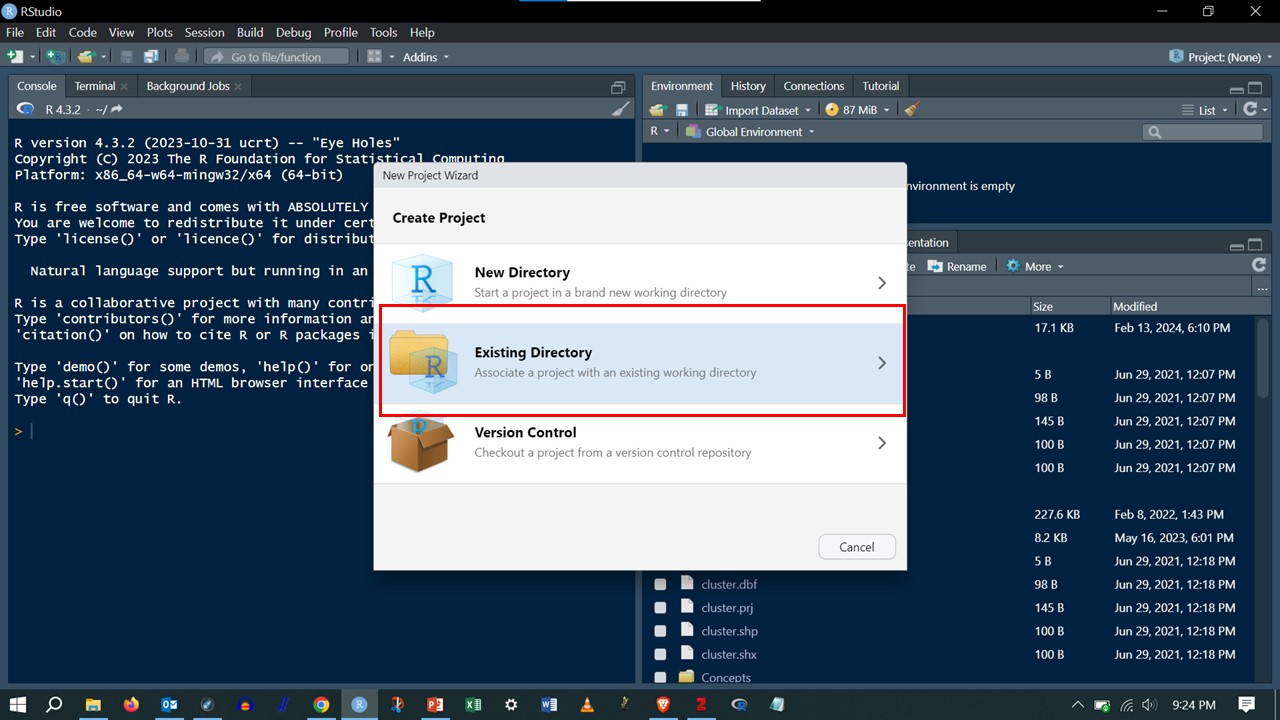
\includegraphics[width=0.7\linewidth]{pictures/Slide8} 

}

\caption{Existing Directory}\label{fig:unnamed-chunk-6}
\end{figure}

\begin{figure}

{\centering 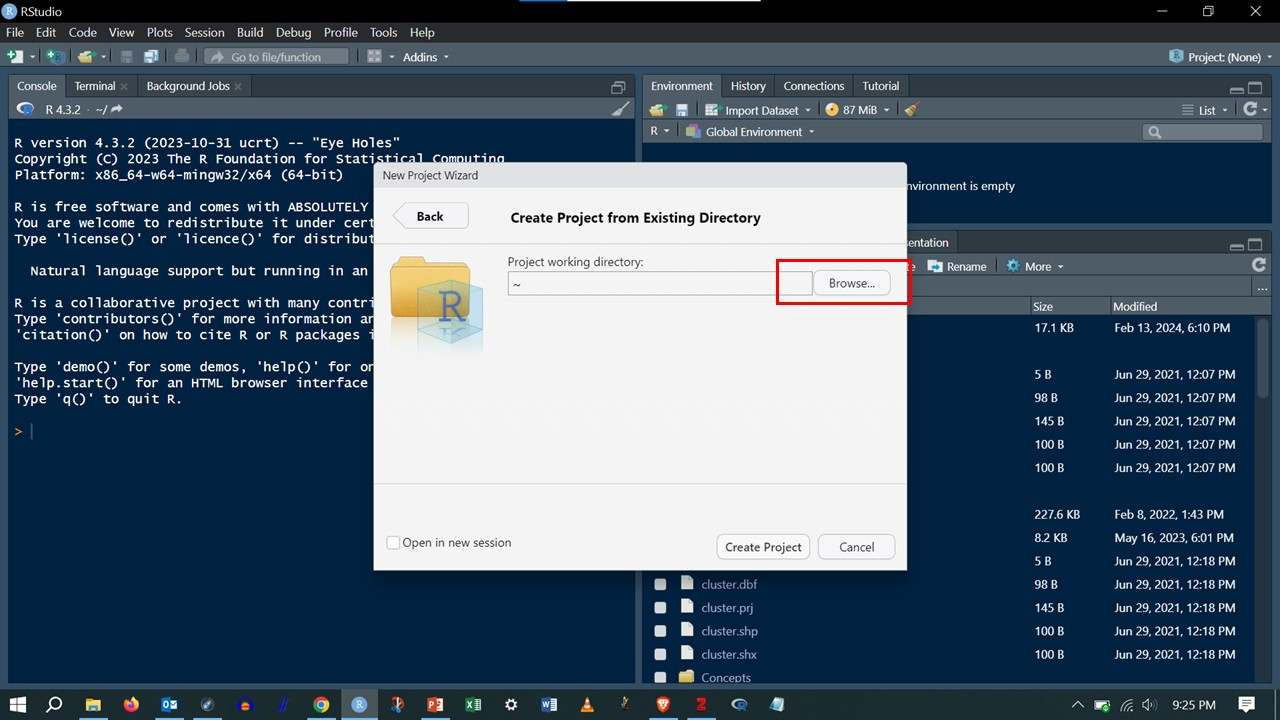
\includegraphics[width=0.7\linewidth]{pictures/Slide9} 

}

\caption{Create}\label{fig:unnamed-chunk-7}
\end{figure}

\begin{figure}

{\centering 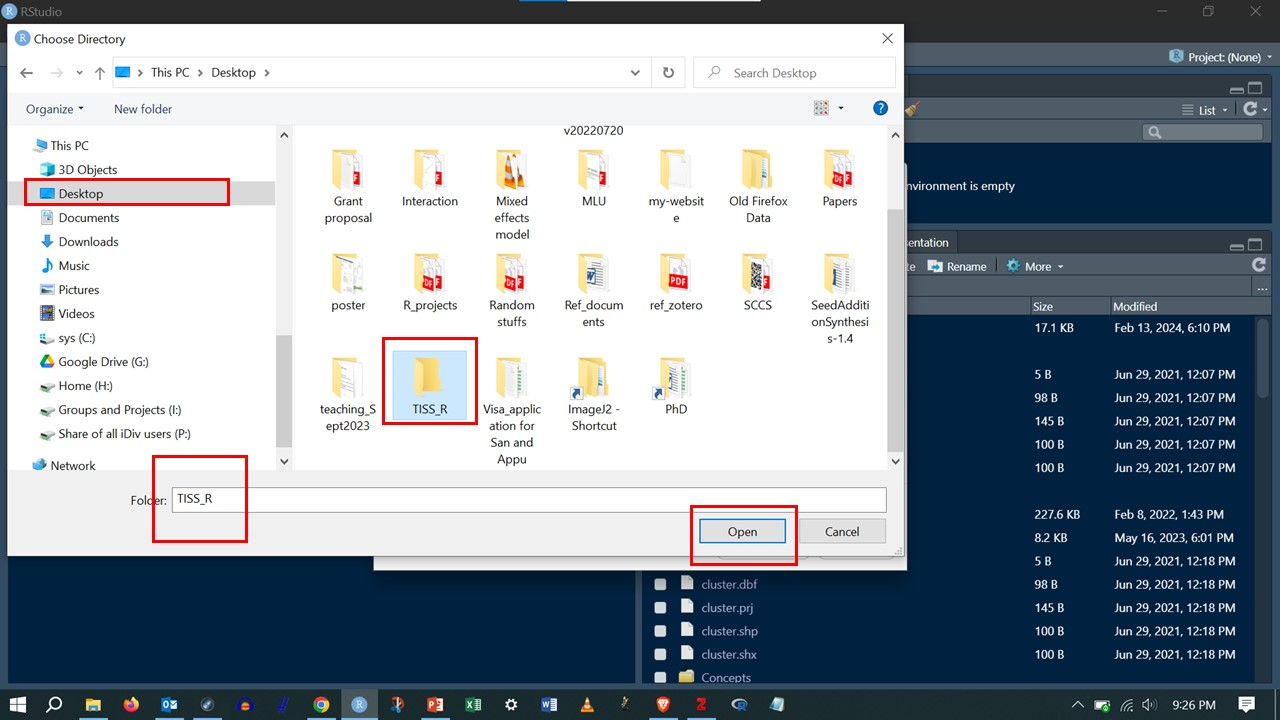
\includegraphics[width=0.7\linewidth]{pictures/Slide10} 

}

\caption{Open}\label{fig:unnamed-chunk-8}
\end{figure}

\begin{figure}

{\centering 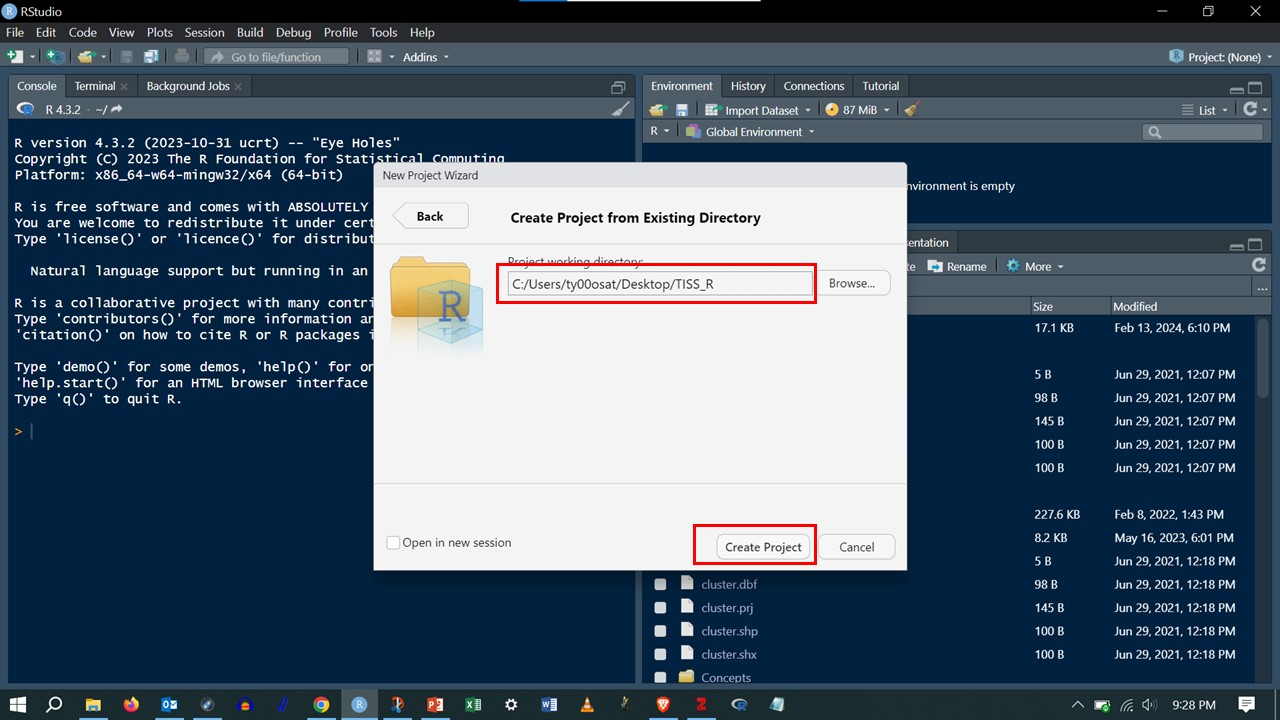
\includegraphics[width=0.7\linewidth]{pictures/Slide11} 

}

\caption{Create Project}\label{fig:unnamed-chunk-9}
\end{figure}

\begin{figure}

{\centering 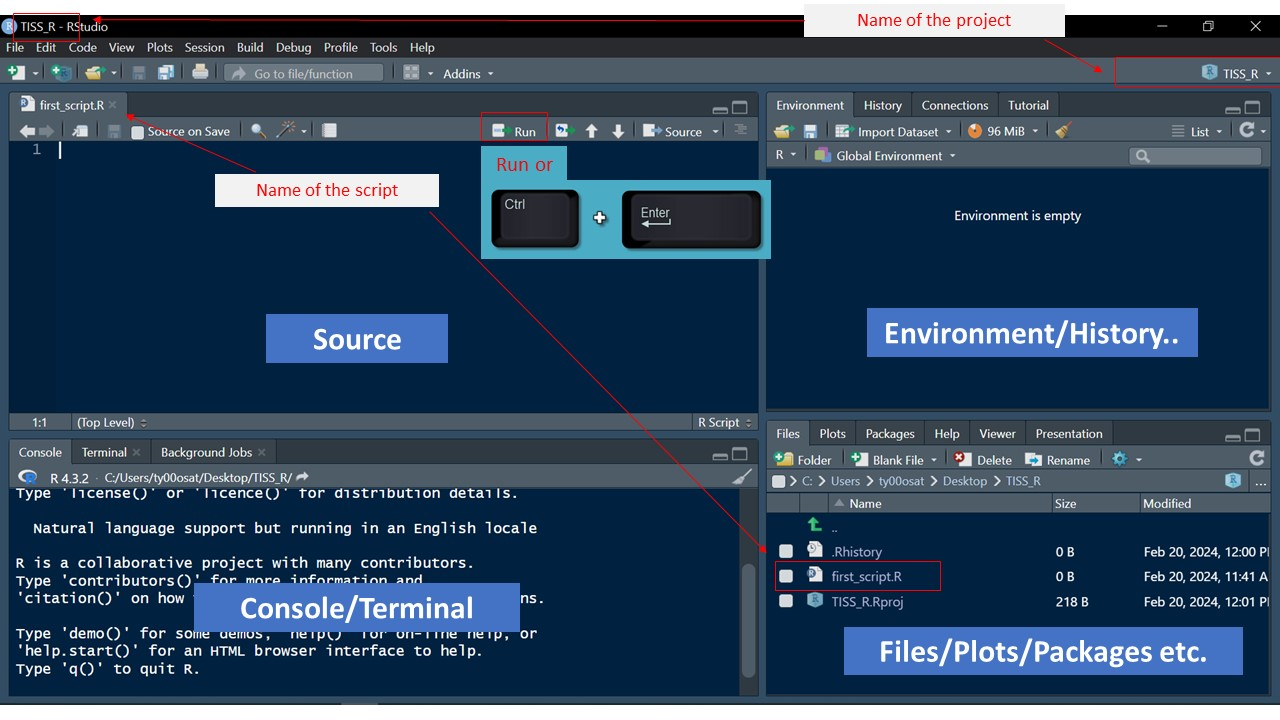
\includegraphics[width=0.7\linewidth]{pictures/Slide12} 

}

\caption{Done: New Project}\label{fig:unnamed-chunk-10}
\end{figure}

\hypertarget{r-operators}{%
\chapter{R operators}\label{r-operators}}

\hypertarget{arithmetic-operators}{%
\section{Arithmetic operators}\label{arithmetic-operators}}

The R arithmetic operators allows us to do math operations, like sums, divisions or multiplications, among others. The following table summarizes all base R arithmetic operators.

\emph{Arithmetic operators}\\
\texttt{+} Plus\\
\texttt{–} Minus\\
\texttt{*} Multiplication\\
\texttt{/} Division\\
\texttt{\^{}} Exponential\\
\texttt{**} Exponential

\emph{Basic operations}

\begin{Shaded}
\begin{Highlighting}[]
\DecValTok{3} \SpecialCharTok{+} \DecValTok{5}   \CommentTok{\# 8}
\end{Highlighting}
\end{Shaded}

\begin{verbatim}
## [1] 8
\end{verbatim}

\begin{Shaded}
\begin{Highlighting}[]
\DecValTok{8} \SpecialCharTok{{-}} \DecValTok{3}   \CommentTok{\# 5}
\end{Highlighting}
\end{Shaded}

\begin{verbatim}
## [1] 5
\end{verbatim}

\begin{Shaded}
\begin{Highlighting}[]
\DecValTok{7} \SpecialCharTok{*} \DecValTok{5}   \CommentTok{\# 35}
\end{Highlighting}
\end{Shaded}

\begin{verbatim}
## [1] 35
\end{verbatim}

\begin{Shaded}
\begin{Highlighting}[]
\DecValTok{1}\SpecialCharTok{/}\DecValTok{2}     \CommentTok{\# 0.5}
\end{Highlighting}
\end{Shaded}

\begin{verbatim}
## [1] 0.5
\end{verbatim}

\begin{Shaded}
\begin{Highlighting}[]
\DecValTok{4} \SpecialCharTok{\^{}} \DecValTok{4}   \CommentTok{\# 256}
\end{Highlighting}
\end{Shaded}

\begin{verbatim}
## [1] 256
\end{verbatim}

\begin{Shaded}
\begin{Highlighting}[]
\DecValTok{4} \SpecialCharTok{**} \DecValTok{4}  \CommentTok{\# 256}
\end{Highlighting}
\end{Shaded}

\begin{verbatim}
## [1] 256
\end{verbatim}

\begin{Shaded}
\begin{Highlighting}[]
\DecValTok{5} \SpecialCharTok{\%\%} \DecValTok{3}  \CommentTok{\# 2}
\end{Highlighting}
\end{Shaded}

\begin{verbatim}
## [1] 2
\end{verbatim}

\begin{Shaded}
\begin{Highlighting}[]
\DecValTok{5} \SpecialCharTok{\%/\%} \DecValTok{3} \CommentTok{\# 1}
\end{Highlighting}
\end{Shaded}

\begin{verbatim}
## [1] 1
\end{verbatim}

\hypertarget{functions}{%
\section{Functions}\label{functions}}

R has many built-in functions. The most common situation is that the function is called by its name using prefix notation, followed by round brackets that enclose the function's arguments (separated by commas if there are multiple arguments). For example, the function round takes a number and, by default, returns the closest integer:

\begin{Shaded}
\begin{Highlighting}[]
\CommentTok{\# the function \textasciigrave{}round\textasciigrave{} takes a number as an argument and }
\CommentTok{\# returns the closest integer (default)}
\FunctionTok{round}\NormalTok{(}\FloatTok{0.6213}\NormalTok{)}
\end{Highlighting}
\end{Shaded}

\begin{verbatim}
## [1] 1
\end{verbatim}

\texttt{round} allows several arguments. It takes as input the number \texttt{x} to be rounded and another integer number digits which gives the number of \texttt{digits} after the comma to which \texttt{x} should be rounded. We can then specify these arguments in a function call of round by providing the named arguments.

\begin{Shaded}
\begin{Highlighting}[]
\FunctionTok{round}\NormalTok{(}\FloatTok{0.6213}\NormalTok{, }\AttributeTok{digits =} \DecValTok{2}\NormalTok{)}
\end{Highlighting}
\end{Shaded}

\begin{verbatim}
## [1] 0.62
\end{verbatim}

Example of another function, \texttt{sum}

\begin{Shaded}
\begin{Highlighting}[]
\FunctionTok{sum}\NormalTok{(}\DecValTok{1}\NormalTok{, }\DecValTok{2}\NormalTok{, }\DecValTok{3}\NormalTok{)}
\end{Highlighting}
\end{Shaded}

\begin{verbatim}
## [1] 6
\end{verbatim}

\hypertarget{reserved-words}{%
\section{Reserved words}\label{reserved-words}}

There are also reserved words you can't use, like \texttt{TRUE}, \texttt{FALSE}, \texttt{NULL}, among others. You can see the full list of R reserved words typing \texttt{help(Reserved)} or \texttt{?Reserved}. It not advisable to use these words outside quotes ('\,', ``\,``) or backtick (`) quotes.

\hypertarget{variables}{%
\section{Variables}\label{variables}}

You can assign values to variables using three assignment operators:\\
\texttt{-\textgreater{}}\strut \\
\texttt{\textless{}-}\strut \\
\texttt{=}

\begin{Shaded}
\begin{Highlighting}[]
\NormalTok{a }\OtherTok{\textless{}{-}} \DecValTok{6}       \CommentTok{\# assigns 6 to variable a}
\DecValTok{7} \OtherTok{{-}\textgreater{}}\NormalTok{ b       }\CommentTok{\# assigns 7 to variable b}
\NormalTok{c }\OtherTok{=} \DecValTok{3}        \CommentTok{\# assigns 3 to variable c, use of = is not widly accepted!}
\NormalTok{d }\OtherTok{\textless{}{-}}\NormalTok{  a }\SpecialCharTok{*}\NormalTok{ b }\SpecialCharTok{/}\NormalTok{ c   }\CommentTok{\# assigns 6 * 7 / 3 = 14 to variable d}
\NormalTok{d           }\CommentTok{\# returns d}
\end{Highlighting}
\end{Shaded}

\begin{verbatim}
## [1] 14
\end{verbatim}

Use \texttt{print()} function to see the output

\texttt{print(a)}\strut \\
\texttt{print(7)}\strut \\
\texttt{print(c)}\strut \\
\texttt{print(d)}

\hypertarget{documenting-code}{%
\section{Documenting code}\label{documenting-code}}

It is good practice to document code with short but informative comments. Comments in R are demarcated with \texttt{\#}.

\begin{Shaded}
\begin{Highlighting}[]
\FunctionTok{round}\NormalTok{(             }\CommentTok{\# call the function \textasciigrave{}round\textasciigrave{}}
  \FunctionTok{sum}\NormalTok{(}\FloatTok{2.213}\SpecialCharTok{*}\FloatTok{3.123}\NormalTok{),}\CommentTok{\# find sum of 2.213*3.123}
  \AttributeTok{digits =} \DecValTok{2}       \CommentTok{\# show the sum with two digits after the \textasciigrave{}.\textasciigrave{}}
\NormalTok{)}
\end{Highlighting}
\end{Shaded}

\begin{verbatim}
## [1] 6.91
\end{verbatim}

In RStudio, you can use Command+Shift+C (on Mac) and Ctrl+Shift+C (on Windows/Linux) to comment or uncomment code, and you can use comments to structure your scripts.
Any comment followed by ---- is treated as a (foldable) section in RStudio.

\begin{Shaded}
\begin{Highlighting}[]
\CommentTok{\# SECTION: variable assignments {-}{-}{-}{-}}
\NormalTok{x }\OtherTok{\textless{}{-}} \DecValTok{6}
\NormalTok{y }\OtherTok{\textless{}{-}} \DecValTok{7}
\end{Highlighting}
\end{Shaded}

\begin{Shaded}
\begin{Highlighting}[]
\CommentTok{\# SECTION: some calculations {-}{-}{-}{-}}

\NormalTok{x }\SpecialCharTok{*}\NormalTok{ y}
\end{Highlighting}
\end{Shaded}

\begin{verbatim}
## [1] 42
\end{verbatim}

\hypertarget{relational-comparison-operators-in-r}{%
\section{Relational / comparison operators in R}\label{relational-comparison-operators-in-r}}

Comparison or relational operators are designed to compare objects and the output of these comparisons are of type boolean. To clarify, the following table summarizes the R relational operators.

Relational operators in R\\
\texttt{\textgreater{}} Greater than\\
\texttt{\textless{}} Lower than\\
\texttt{\textgreater{}=} Greater or equal than\\
\texttt{\textless{}=} Lower or equal than\\
\texttt{==} Equal to\\
\texttt{!=} Not equal to

\begin{Shaded}
\begin{Highlighting}[]
\DecValTok{3} \SpecialCharTok{\textgreater{}} \DecValTok{5}  \CommentTok{\# FALSE}
\end{Highlighting}
\end{Shaded}

\begin{verbatim}
## [1] FALSE
\end{verbatim}

\begin{Shaded}
\begin{Highlighting}[]
\DecValTok{3} \SpecialCharTok{\textless{}} \DecValTok{5}  \CommentTok{\# TRUE}
\end{Highlighting}
\end{Shaded}

\begin{verbatim}
## [1] TRUE
\end{verbatim}

\begin{Shaded}
\begin{Highlighting}[]
\DecValTok{3} \SpecialCharTok{\textgreater{}=} \DecValTok{5} \CommentTok{\# FALSE}
\end{Highlighting}
\end{Shaded}

\begin{verbatim}
## [1] FALSE
\end{verbatim}

\begin{Shaded}
\begin{Highlighting}[]
\DecValTok{3} \SpecialCharTok{\textless{}=} \DecValTok{5} \CommentTok{\# TRUE}
\end{Highlighting}
\end{Shaded}

\begin{verbatim}
## [1] TRUE
\end{verbatim}

\begin{Shaded}
\begin{Highlighting}[]
\DecValTok{3} \SpecialCharTok{==} \DecValTok{5} \CommentTok{\# FALSE}
\end{Highlighting}
\end{Shaded}

\begin{verbatim}
## [1] FALSE
\end{verbatim}

\begin{Shaded}
\begin{Highlighting}[]
\DecValTok{3} \SpecialCharTok{!=} \DecValTok{5} \CommentTok{\# TRUE}
\end{Highlighting}
\end{Shaded}

\begin{verbatim}
## [1] TRUE
\end{verbatim}

\hypertarget{data-types}{%
\section{Data types}\label{data-types}}

To learn a programming language entails to first learn something about what kinds of objects we will have to deal with. Let's therefore briefly go through the data types. We can assess the type of an object stored in variable \texttt{x} with the function \texttt{typeof(x)}.

\begin{Shaded}
\begin{Highlighting}[]
\NormalTok{x }\OtherTok{\textless{}{-}} \DecValTok{1}
\FunctionTok{typeof}\NormalTok{(x)}
\end{Highlighting}
\end{Shaded}

\begin{verbatim}
## [1] "double"
\end{verbatim}

\begin{Shaded}
\begin{Highlighting}[]
\NormalTok{x }\OtherTok{\textless{}{-}} \StringTok{"hello"}
\FunctionTok{typeof}\NormalTok{(x)}
\end{Highlighting}
\end{Shaded}

\begin{verbatim}
## [1] "character"
\end{verbatim}

\begin{Shaded}
\begin{Highlighting}[]
\NormalTok{x }\OtherTok{\textless{}{-}} \ConstantTok{TRUE}
\FunctionTok{typeof}\NormalTok{(x)}
\end{Highlighting}
\end{Shaded}

\begin{verbatim}
## [1] "logical"
\end{verbatim}

\begin{Shaded}
\begin{Highlighting}[]
\NormalTok{x }\OtherTok{\textless{}{-}}\NormalTok{ mean}
\FunctionTok{typeof}\NormalTok{(x)}
\end{Highlighting}
\end{Shaded}

\begin{verbatim}
## [1] "closure"
\end{verbatim}

It is possible to cast objects of one type into another type using functions \texttt{as.} in base R.

\begin{Shaded}
\begin{Highlighting}[]
\NormalTok{x }\OtherTok{\textless{}{-}} \FunctionTok{as.numeric}\NormalTok{(}\DecValTok{1}\NormalTok{) }\CommentTok{\# "double"}
\FunctionTok{typeof}\NormalTok{(x) }
\end{Highlighting}
\end{Shaded}

\begin{verbatim}
## [1] "double"
\end{verbatim}

\begin{Shaded}
\begin{Highlighting}[]
\NormalTok{x }\OtherTok{\textless{}{-}} \FunctionTok{as.character}\NormalTok{(}\DecValTok{1}\NormalTok{) }\CommentTok{\# "character"}
\FunctionTok{typeof}\NormalTok{(x)}
\end{Highlighting}
\end{Shaded}

\begin{verbatim}
## [1] "character"
\end{verbatim}

\hypertarget{installing-r-packages}{%
\chapter{Installing R packages}\label{installing-r-packages}}

\hypertarget{package}{%
\section{Package}\label{package}}

An R package is a library of functions that have been developed to cover some needs or specific scientific methods that are not implemented in base R.

The Comprehensive R Archive Network (CRAN) is the official R packages repository, with thousands of free R packages available. Most of them have been developed by Data Scientists, Statisticians, Professors and researchers.

First, you need to look for the name of the package you want to install. You may want to research for your topic googling something like: `graphics package R' or `R package for time series'.

Once you decided what package to install, just call the \texttt{install.packages} function with the name of the package inside the parenthesis \texttt{()} with quotation marks \texttt{"\ "} or \texttt{\textquotesingle{}\ \textquotesingle{}}. As an example, we are going to install the \texttt{calendR} package, that allows creating monthly and yearly calendars, but you can install the package you prefer.

\begin{Shaded}
\begin{Highlighting}[]
\CommentTok{\# install.packages(\textquotesingle{}calendR\textquotesingle{})}
\end{Highlighting}
\end{Shaded}

Once you see a similar looking message in the Console ``The downloaded binary packages are in''drive user downloaded\_packages'', it is good idea to add a comment \texttt{\#} before install.packages like this \texttt{\#\ install.packages(\textquotesingle{}calendR\textquotesingle{})} to avoid installing the same package again and again!

After installation, you need to load the package if you want to access its functions. For that purpose, you can load it with the \texttt{library} function, specifying the package name with or without quotation marks.

\begin{Shaded}
\begin{Highlighting}[]
\FunctionTok{library}\NormalTok{(calendR)}
\end{Highlighting}
\end{Shaded}

\begin{verbatim}
## ~~ Package calendR
## Visit https://r-coder.com/ for R tutorials ~~
\end{verbatim}

Once loaded, you can use \texttt{?} or the \texttt{help} function with the package name or the name of any function to see the documentation. You will also find useful examples to understand how the package works.

\texttt{?calendR}\strut \\
\texttt{help("calendR")}\strut \\
\texttt{help(calendR)}

In addition, you can find out where the packages are going to be installed calling the \texttt{.libPaths()} function.

\begin{Shaded}
\begin{Highlighting}[]
\FunctionTok{.libPaths}\NormalTok{()}
\end{Highlighting}
\end{Shaded}

\begin{verbatim}
## [1] "C:/Users/ty00osat/Documents/R-4.3.2/library"
\end{verbatim}

Alternatively, you can install R packages from the menu (Package).

\begin{figure}

{\centering 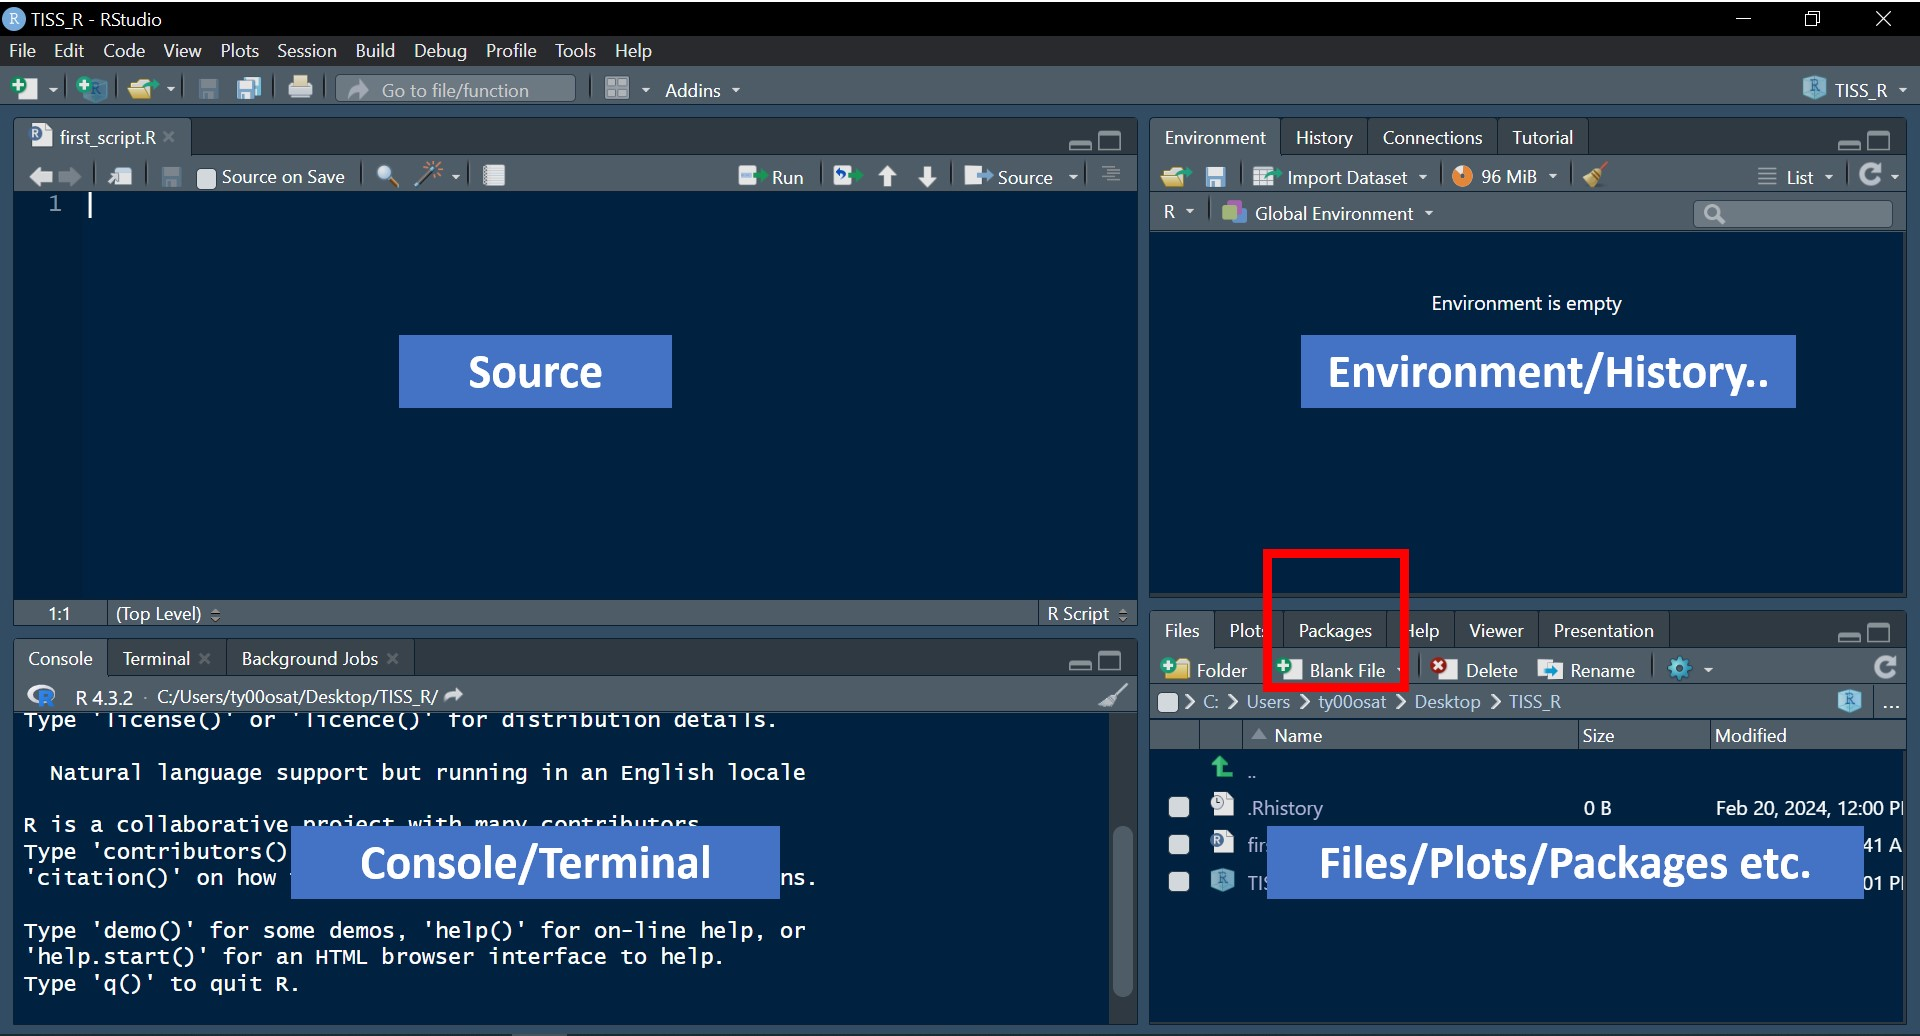
\includegraphics[width=0.7\linewidth]{pictures/Package panel} 

}

\caption{Package}\label{fig:unnamed-chunk-25}
\end{figure}

In RStudio go to Tools → Install Packages and in the Install from option select Repository (CRAN) and then specify the packages you want.

If you need to install several packages at once without writing the same function over and over again, you can make use of the c function within the \texttt{install.packages} function. Note that now the quotation marks are needed to specify the packages names.

\texttt{install.packages(c("ggplot2",\ "dplyr"))}

Once installed, you can get a list of all the functions in the package. If the package is on CRAN, you will find documentation in PDF format of all functions inside a page like \url{https://cran.r-project.org/web/packages/package_name}. Recall you can access this documentation in HTML format with the help function.

\texttt{help(package\ =\ ggplot2)}

\hypertarget{vectors-matrices}{%
\chapter{Vectors \& matrices}\label{vectors-matrices}}

R is essentially an array-based language. Arrays are arbitrary but finite-dimensional matrices.\\
* vectors = one-dimensional arrays\\
* matrices = two-dimensional arrays\\
* arrays = more-than-two-dimensional, it is important to keep in mind that arrays can contain objects of other types than numeric information (as long as all objects in the array are of the same type).

\hypertarget{numeric-vector}{%
\section{Numeric vector}\label{numeric-vector}}

\begin{Shaded}
\begin{Highlighting}[]
\NormalTok{x }\OtherTok{\textless{}{-}} \DecValTok{1}
\FunctionTok{print}\NormalTok{(x)}
\end{Highlighting}
\end{Shaded}

\begin{verbatim}
## [1] 1
\end{verbatim}

Vectors in general can be declared with the built-in function \texttt{c()}. To memorize this, think of concatenation or combination.

There are also helpful functions to generate sequences of numbers:

\begin{Shaded}
\begin{Highlighting}[]
\NormalTok{x }\OtherTok{\textless{}{-}} \FunctionTok{seq}\NormalTok{(}\DecValTok{1}\SpecialCharTok{:}\DecValTok{10}\NormalTok{)}
\NormalTok{x }\CommentTok{\# or}
\end{Highlighting}
\end{Shaded}

\begin{verbatim}
##  [1]  1  2  3  4  5  6  7  8  9 10
\end{verbatim}

\begin{Shaded}
\begin{Highlighting}[]
\FunctionTok{print}\NormalTok{(x)}
\end{Highlighting}
\end{Shaded}

\begin{verbatim}
##  [1]  1  2  3  4  5  6  7  8  9 10
\end{verbatim}

\hypertarget{mathematical-operation}{%
\section{Mathematical operation}\label{mathematical-operation}}

Every mathematical operation can be expected to apply to a vector.

\begin{Shaded}
\begin{Highlighting}[]
\NormalTok{a }\OtherTok{\textless{}{-}} \FunctionTok{c}\NormalTok{(}\DecValTok{2}\NormalTok{, }\DecValTok{4}\NormalTok{, }\DecValTok{6}\NormalTok{, }\DecValTok{8}\NormalTok{) }
\NormalTok{a}\SpecialCharTok{+}\DecValTok{1}
\end{Highlighting}
\end{Shaded}

\begin{verbatim}
## [1] 3 5 7 9
\end{verbatim}

\begin{Shaded}
\begin{Highlighting}[]
\NormalTok{a}\SpecialCharTok{*}\DecValTok{4}
\end{Highlighting}
\end{Shaded}

\begin{verbatim}
## [1]  8 16 24 32
\end{verbatim}

\begin{Shaded}
\begin{Highlighting}[]
\NormalTok{a}\SpecialCharTok{/}\FloatTok{0.5}
\end{Highlighting}
\end{Shaded}

\begin{verbatim}
## [1]  4  8 12 16
\end{verbatim}

\begin{Shaded}
\begin{Highlighting}[]
\NormalTok{b }\OtherTok{\textless{}{-}} \FunctionTok{c}\NormalTok{(}\DecValTok{8}\NormalTok{, }\DecValTok{6}\NormalTok{, }\DecValTok{4}\NormalTok{, }\DecValTok{2}\NormalTok{) }

\NormalTok{a}\SpecialCharTok{+}\NormalTok{b}
\end{Highlighting}
\end{Shaded}

\begin{verbatim}
## [1] 10 10 10 10
\end{verbatim}

\begin{Shaded}
\begin{Highlighting}[]
\NormalTok{a}\SpecialCharTok{*}\NormalTok{b}
\end{Highlighting}
\end{Shaded}

\begin{verbatim}
## [1] 16 24 24 16
\end{verbatim}

\hypertarget{indexing}{%
\section{Indexing}\label{indexing}}

Indexing in R starts with 1, not 0.

\begin{Shaded}
\begin{Highlighting}[]
\NormalTok{x }\OtherTok{\textless{}{-}} \FunctionTok{c}\NormalTok{(}\DecValTok{2}\NormalTok{, }\DecValTok{4}\NormalTok{, }\DecValTok{6}\NormalTok{, }\DecValTok{8}\NormalTok{)   }\CommentTok{\# this is now a 4{-}place vector}
\NormalTok{x}
\end{Highlighting}
\end{Shaded}

\begin{verbatim}
## [1] 2 4 6 8
\end{verbatim}

\begin{Shaded}
\begin{Highlighting}[]
\NormalTok{x[}\DecValTok{2}\NormalTok{] }\CommentTok{\# what is the entry in position 2 of the vector x?}
\end{Highlighting}
\end{Shaded}

\begin{verbatim}
## [1] 4
\end{verbatim}

\begin{Shaded}
\begin{Highlighting}[]
\NormalTok{x[}\DecValTok{1}\NormalTok{] }\CommentTok{\# what is the entry in position 1 of the vector x?}
\end{Highlighting}
\end{Shaded}

\begin{verbatim}
## [1] 2
\end{verbatim}

\hypertarget{numeric-matrices}{%
\section{Numeric matrices}\label{numeric-matrices}}

\begin{Shaded}
\begin{Highlighting}[]
\NormalTok{x }\OtherTok{\textless{}{-}} \FunctionTok{seq}\NormalTok{(}\DecValTok{1}\SpecialCharTok{:}\DecValTok{10}\NormalTok{)}
\NormalTok{m1 }\OtherTok{\textless{}{-}} \FunctionTok{matrix}\NormalTok{(x)}
\NormalTok{m1}
\end{Highlighting}
\end{Shaded}

\begin{verbatim}
##       [,1]
##  [1,]    1
##  [2,]    2
##  [3,]    3
##  [4,]    4
##  [5,]    5
##  [6,]    6
##  [7,]    7
##  [8,]    8
##  [9,]    9
## [10,]   10
\end{verbatim}

\begin{Shaded}
\begin{Highlighting}[]
\NormalTok{m }\OtherTok{\textless{}{-}} \FunctionTok{matrix}\NormalTok{(}\DecValTok{1}\SpecialCharTok{:}\DecValTok{6}\NormalTok{, }\AttributeTok{ncol =} \DecValTok{3}\NormalTok{)}
\NormalTok{m}
\end{Highlighting}
\end{Shaded}

\begin{verbatim}
##      [,1] [,2] [,3]
## [1,]    1    3    5
## [2,]    2    4    6
\end{verbatim}

\hypertarget{names-for-vectors-matrices-and-arrays}{%
\section{Names for vectors, matrices and arrays}\label{names-for-vectors-matrices-and-arrays}}

The positions in a vector can be given names. These names of vector \texttt{x} positions are retrieved and set by the \texttt{names} function.

\begin{Shaded}
\begin{Highlighting}[]
\NormalTok{students }\OtherTok{\textless{}{-}} \FunctionTok{c}\NormalTok{(}\StringTok{"Prachi"}\NormalTok{, }\StringTok{"Rishi"}\NormalTok{, }\StringTok{"Soumya"}\NormalTok{)  }\CommentTok{\# names of students}
\NormalTok{grades }\OtherTok{\textless{}{-}} \FunctionTok{c}\NormalTok{(}\FloatTok{1.3}\NormalTok{, }\FloatTok{2.7}\NormalTok{, }\FloatTok{2.0}\NormalTok{)              }\CommentTok{\# a vector of grades}

\FunctionTok{names}\NormalTok{(grades) }\OtherTok{\textless{}{-}}\NormalTok{ students  }\CommentTok{\# assign names}
\FunctionTok{names}\NormalTok{(grades)              }\CommentTok{\# retrieve names again: names assigned}
\end{Highlighting}
\end{Shaded}

\begin{verbatim}
## [1] "Prachi" "Rishi"  "Soumya"
\end{verbatim}

\hypertarget{characters-or-strings}{%
\section{Characters or strings}\label{characters-or-strings}}

Strings are called characters in R. We will be stubborn and call them strings for most of the time here. We can assign a string value to a variable by putting the string in double-quotes.

\begin{Shaded}
\begin{Highlighting}[]
\NormalTok{institute }\OtherTok{\textless{}{-}} \StringTok{\textquotesingle{}TISS\textquotesingle{}}
\FunctionTok{typeof}\NormalTok{(institute)}
\end{Highlighting}
\end{Shaded}

\begin{verbatim}
## [1] "character"
\end{verbatim}

\begin{Shaded}
\begin{Highlighting}[]
\FunctionTok{print}\NormalTok{(institute)}
\end{Highlighting}
\end{Shaded}

\begin{verbatim}
## [1] "TISS"
\end{verbatim}

Create vectors of characters

\begin{Shaded}
\begin{Highlighting}[]
\NormalTok{chr\_vector }\OtherTok{\textless{}{-}} \FunctionTok{c}\NormalTok{(}\StringTok{"small"}\NormalTok{, }\StringTok{"medium"}\NormalTok{, }\StringTok{"large"}\NormalTok{)}
\FunctionTok{print}\NormalTok{(chr\_vector)}
\end{Highlighting}
\end{Shaded}

\begin{verbatim}
## [1] "small"  "medium" "large"
\end{verbatim}

\begin{Shaded}
\begin{Highlighting}[]
\NormalTok{chr\_vector}
\end{Highlighting}
\end{Shaded}

\begin{verbatim}
## [1] "small"  "medium" "large"
\end{verbatim}

\begin{Shaded}
\begin{Highlighting}[]
\FunctionTok{typeof}\NormalTok{(chr\_vector)}
\end{Highlighting}
\end{Shaded}

\begin{verbatim}
## [1] "character"
\end{verbatim}

Factors are special vectors, which treat their elements as instances of a finite set of categories.

\begin{Shaded}
\begin{Highlighting}[]
\NormalTok{factor\_vector }\OtherTok{\textless{}{-}} \FunctionTok{as.factor}\NormalTok{(}\FunctionTok{c}\NormalTok{(}\StringTok{"small"}\NormalTok{, }\StringTok{"medium"}\NormalTok{, }\StringTok{"large"}\NormalTok{))}
\FunctionTok{print}\NormalTok{(factor\_vector)}
\end{Highlighting}
\end{Shaded}

\begin{verbatim}
## [1] small  medium large 
## Levels: large medium small
\end{verbatim}

\begin{Shaded}
\begin{Highlighting}[]
\NormalTok{factor\_vector}
\end{Highlighting}
\end{Shaded}

\begin{verbatim}
## [1] small  medium large 
## Levels: large medium small
\end{verbatim}

\begin{Shaded}
\begin{Highlighting}[]
\FunctionTok{typeof}\NormalTok{(factor\_vector)}
\end{Highlighting}
\end{Shaded}

\begin{verbatim}
## [1] "integer"
\end{verbatim}

\begin{Shaded}
\begin{Highlighting}[]
\FunctionTok{levels}\NormalTok{(factor\_vector) }\CommentTok{\# alphabetically ordered}
\end{Highlighting}
\end{Shaded}

\begin{verbatim}
## [1] "large"  "medium" "small"
\end{verbatim}

A factor in R is a data structure used to represent a vector as categorical data. Therefore, the factor object takes a bounded number of different values called levels. Factors are very useful when working with character columns of data frames, for creating barplots and creating statistical summaries for categorical variables.

For plotting or other representational purposes, it can help to manually specify an ordering on the \texttt{levels} of a factor using the levels argument.

\begin{Shaded}
\begin{Highlighting}[]
\FunctionTok{factor}\NormalTok{(factor\_vector, }\AttributeTok{levels =} \FunctionTok{c}\NormalTok{(}\StringTok{\textquotesingle{}large\textquotesingle{}}\NormalTok{, }\StringTok{\textquotesingle{}medium\textquotesingle{}}\NormalTok{, }\StringTok{\textquotesingle{}small\textquotesingle{}}\NormalTok{))}
\end{Highlighting}
\end{Shaded}

\begin{verbatim}
## [1] small  medium large 
## Levels: large medium small
\end{verbatim}

\begin{Shaded}
\begin{Highlighting}[]
\FunctionTok{levels}\NormalTok{(factor\_vector) }\CommentTok{\# ordered the way we want}
\end{Highlighting}
\end{Shaded}

\begin{verbatim}
## [1] "large"  "medium" "small"
\end{verbatim}

\begin{Shaded}
\begin{Highlighting}[]
\NormalTok{days }\OtherTok{\textless{}{-}} \FunctionTok{c}\NormalTok{(}\StringTok{"Friday"}\NormalTok{, }\StringTok{"Tuesday"}\NormalTok{, }\StringTok{"Thursday"}\NormalTok{, }\StringTok{"Monday"}\NormalTok{, }\StringTok{"Wednesday"}\NormalTok{, }\StringTok{"Monday"}\NormalTok{,}
          \StringTok{"Wednesday"}\NormalTok{, }\StringTok{"Monday"}\NormalTok{, }\StringTok{"Monday"}\NormalTok{, }\StringTok{"Wednesday"}\NormalTok{, }\StringTok{"Sunday"}\NormalTok{, }\StringTok{"Saturday"}\NormalTok{)}

\CommentTok{\# Levels in alphabetical order}
\NormalTok{my\_factor }\OtherTok{\textless{}{-}} \FunctionTok{factor}\NormalTok{(days)}
\NormalTok{my\_factor}
\end{Highlighting}
\end{Shaded}

\begin{verbatim}
##  [1] Friday    Tuesday   Thursday  Monday    Wednesday Monday    Wednesday
##  [8] Monday    Monday    Wednesday Sunday    Saturday 
## Levels: Friday Monday Saturday Sunday Thursday Tuesday Wednesday
\end{verbatim}

Convert numeric to factor in R.\\
Suppose you have registered the birth city of six individuals with the following codification:
1. Mumbai
2. Chennai
3. Bangalore
3. Cochin\\
Hence, you will have something like the following data stored in a numeric vector:

\begin{Shaded}
\begin{Highlighting}[]
\CommentTok{\# Sample data}
\NormalTok{city }\OtherTok{\textless{}{-}} \FunctionTok{c}\NormalTok{(}\DecValTok{3}\NormalTok{, }\DecValTok{2}\NormalTok{, }\DecValTok{1}\NormalTok{, }\DecValTok{4}\NormalTok{, }\DecValTok{3}\NormalTok{, }\DecValTok{2}\NormalTok{)}
\end{Highlighting}
\end{Shaded}

Now, you can call the \texttt{factor} to convert the data into factor and get it categorized for further analysis.

\begin{Shaded}
\begin{Highlighting}[]
\NormalTok{my\_factor }\OtherTok{\textless{}{-}} \FunctionTok{factor}\NormalTok{(city)}
\NormalTok{my\_factor}
\end{Highlighting}
\end{Shaded}

\begin{verbatim}
## [1] 3 2 1 4 3 2
## Levels: 1 2 3 4
\end{verbatim}

If the input vector is numeric, as in the previous section, the corresponding label (the city) is not reflected. In order to solve this issue, you can store the data in a factor object using the \texttt{factor} function and indicate the corresponding \texttt{labels} of the levels in the labels argument, in order to rename the factor \texttt{levels}.

\begin{Shaded}
\begin{Highlighting}[]
\CommentTok{\# Setting the labels in the corresponding order}
\NormalTok{factor\_cities }\OtherTok{\textless{}{-}} \FunctionTok{factor}\NormalTok{(city, }\AttributeTok{labels =} \FunctionTok{c}\NormalTok{(}\StringTok{"Mumbai"}\NormalTok{, }\StringTok{"Chennai"}\NormalTok{, }\StringTok{"Bangalore"}\NormalTok{, }\StringTok{"Cochin"}\NormalTok{))}

\CommentTok{\# Print the result}
\NormalTok{factor\_cities}
\end{Highlighting}
\end{Shaded}

\begin{verbatim}
## [1] Bangalore Chennai   Mumbai    Cochin    Bangalore Chennai  
## Levels: Mumbai Chennai Bangalore Cochin
\end{verbatim}

\hypertarget{list-data-frame}{%
\chapter{List \& Data frame}\label{list-data-frame}}

Lists are very important in R because almost all structured data that belongs together is stored as lists. Objects are special kinds of lists. Data is stored in special kinds of lists, so-called data frames or so-called tibbles.

A data frame is base R's standard format to store data in. A data frame is a list of vectors of equal length. Data sets are instantiated with the function \texttt{data.frame}.

\hypertarget{making-a-data-frame}{%
\section{Making a data frame}\label{making-a-data-frame}}

\begin{Shaded}
\begin{Highlighting}[]
\NormalTok{name }\OtherTok{=} \FunctionTok{c}\NormalTok{(}\StringTok{"saneesh"}\NormalTok{, }\StringTok{"sanusha"}\NormalTok{, }\StringTok{"appu"}\NormalTok{, }\StringTok{"jaru"}\NormalTok{)}
\NormalTok{sex }\OtherTok{=} \FunctionTok{c}\NormalTok{(}\DecValTok{2}\NormalTok{, }\DecValTok{0}\NormalTok{, }\DecValTok{5}\NormalTok{, }\DecValTok{8}\NormalTok{)}

\NormalTok{df }\OtherTok{\textless{}{-}} \FunctionTok{data.frame}\NormalTok{(name, sex)}

\NormalTok{df }\OtherTok{\textless{}{-}} \CommentTok{\# df= data frame}
  \FunctionTok{data.frame}\NormalTok{(}\AttributeTok{name =} \FunctionTok{c}\NormalTok{(}\StringTok{"saneesh"}\NormalTok{, }\StringTok{"sanusha"}\NormalTok{, }\StringTok{"appu"}\NormalTok{, }\StringTok{"jaru"}\NormalTok{),}
             \AttributeTok{sex =} \FunctionTok{c}\NormalTok{(}\DecValTok{2}\NormalTok{, }\DecValTok{0}\NormalTok{, }\DecValTok{5}\NormalTok{, }\DecValTok{8}\NormalTok{))}
\end{Highlighting}
\end{Shaded}

\hypertarget{names-functions}{%
\chapter{Names functions}\label{names-functions}}

The special operator supplied by base R to create new function is the keyword \texttt{function}. Here is an example of defining a new function with two input variables \texttt{x} and \texttt{y} that returns a computation based on these numbers. We assign a newly created function to the variable cool\_function so that we can use this name to call the function later. Notice that the use of the return keyword is optional here. If it is left out, the evaluation of the last line is returned.

\begin{Shaded}
\begin{Highlighting}[]
\CommentTok{\# define a new function}
\CommentTok{\# {-} takes two numbers x \& y as argument}
\CommentTok{\# {-} returns x + y}

\NormalTok{sum\_function }\OtherTok{\textless{}{-}} \ControlFlowTok{function}\NormalTok{(x, y) \{}
\NormalTok{  z }\OtherTok{=}\NormalTok{ x }\SpecialCharTok{+}\NormalTok{ y}
  \FunctionTok{return}\NormalTok{(z)}
\NormalTok{\}}

\FunctionTok{sum\_function}\NormalTok{(}\AttributeTok{x =} \DecValTok{1}\NormalTok{, }\AttributeTok{y =} \DecValTok{4}\NormalTok{)}
\end{Highlighting}
\end{Shaded}

\begin{verbatim}
## [1] 5
\end{verbatim}

\begin{Shaded}
\begin{Highlighting}[]
\FunctionTok{sum\_function}\NormalTok{(}\DecValTok{12}\NormalTok{, }\DecValTok{4}\NormalTok{)}
\end{Highlighting}
\end{Shaded}

\begin{verbatim}
## [1] 16
\end{verbatim}

\begin{Shaded}
\begin{Highlighting}[]
\CommentTok{\# define a new function}
\CommentTok{\# we know x and total we want to calculate percentage}

\NormalTok{percentage\_function }\OtherTok{\textless{}{-}} \ControlFlowTok{function}\NormalTok{(x, y) \{}
\NormalTok{  percentage }\OtherTok{=}\NormalTok{ (x }\SpecialCharTok{/}\NormalTok{ y)}\SpecialCharTok{*}\DecValTok{100}
  \FunctionTok{return}\NormalTok{(percentage)}
\NormalTok{\}}

\FunctionTok{percentage\_function}\NormalTok{ (}\DecValTok{360}\NormalTok{, }\DecValTok{600}\NormalTok{)}
\end{Highlighting}
\end{Shaded}

\begin{verbatim}
## [1] 60
\end{verbatim}

\begin{Shaded}
\begin{Highlighting}[]
\CommentTok{\# we know percentage and total we want to calculate x}

\NormalTok{reverse\_percentage\_function }\OtherTok{\textless{}{-}} \ControlFlowTok{function}\NormalTok{(x, y) \{}
\NormalTok{  percentage }\OtherTok{=}\NormalTok{ (x }\SpecialCharTok{/} \DecValTok{100}\NormalTok{)}\SpecialCharTok{*}\NormalTok{y}
  \FunctionTok{return}\NormalTok{(percentage)}
\NormalTok{\}}

\FunctionTok{reverse\_percentage\_function}\NormalTok{ (}\DecValTok{60}\NormalTok{, }\DecValTok{600}\NormalTok{)}
\end{Highlighting}
\end{Shaded}

\begin{verbatim}
## [1] 360
\end{verbatim}

\hypertarget{loops-and-maps}{%
\section{Loops and maps}\label{loops-and-maps}}

\hypertarget{import-data}{%
\chapter{Import data}\label{import-data}}

\hypertarget{importing-from-.csv-file}{%
\section{Importing from .csv file}\label{importing-from-.csv-file}}

Although creating data frames from existing data structures is extremely useful, by far the most common approach is to create a data frame by importing data from an external file. To do this, you'll need to have your data correctly formatted and saved in a file format that R is able to recognize. Fortunately for us, R is able to recognize a wide variety of file formats, although in reality you'll probably end up only using two or three regularly.\\
\emph{Saving files to import}
The easiest method of creating a data file to import into R is to enter your data into a spreadsheet using either Microsoft Excel or LibreOffice Calc and save the spreadsheet as a comma delimited file.
To save a spreadsheet as a comma delimited file in Microsoft Excel or LibreOffice Calc select File -\textgreater{} Save as \ldots{} from the main menu. You will need to specify the location (project folder) you want to save your file in the `Save in folder' option and the name of the file in the `Name' option. In the drop down menu located above the `Save' button change the default `Save as type:' to 'CSV(Comma delimited) (*.csv)'.

Once you've saved your data file in a suitable format we can now read this file into R.

If you don't have a \texttt{*.csv} don't worry, we will make one using the \texttt{write.csv} function.

\begin{Shaded}
\begin{Highlighting}[]
\NormalTok{df }\OtherTok{\textless{}{-}} \CommentTok{\# df= data frame}
  \FunctionTok{data.frame}\NormalTok{(}\AttributeTok{name =} \FunctionTok{c}\NormalTok{(}\StringTok{"saneesh"}\NormalTok{, }\StringTok{"sanusha"}\NormalTok{, }\StringTok{"appu"}\NormalTok{, }\StringTok{"jaru"}\NormalTok{),}
             \AttributeTok{sex =} \FunctionTok{c}\NormalTok{(}\DecValTok{2}\NormalTok{, }\DecValTok{0}\NormalTok{, }\DecValTok{5}\NormalTok{, }\DecValTok{8}\NormalTok{),}
             \AttributeTok{height =} \FunctionTok{c}\NormalTok{(}\DecValTok{167}\NormalTok{, }\DecValTok{158}\NormalTok{, }\DecValTok{110}\NormalTok{, }\DecValTok{50}\NormalTok{))}

\CommentTok{\# copy the name of the data frame \textasciigrave{}df\textasciigrave{}}

\FunctionTok{write.csv}\NormalTok{(df, }\CommentTok{\# copied name}
          \AttributeTok{file=} \StringTok{\textquotesingle{}family.csv\textquotesingle{}}\NormalTok{, }\CommentTok{\# a new file will be made in the project folder with name family.csv. Go check after running the code!}
          \AttributeTok{row.names =} \ConstantTok{FALSE}\NormalTok{) }\CommentTok{\# to avoid auto generated row names}
\end{Highlighting}
\end{Shaded}

\hypertarget{read-.csv}{%
\section{Read .csv}\label{read-.csv}}

Now to read the newly created \texttt{family.csv} file to \texttt{R} or any other file there are many ways.

\begin{Shaded}
\begin{Highlighting}[]
\NormalTok{family }\OtherTok{\textless{}{-}} \FunctionTok{read.csv}\NormalTok{(}\AttributeTok{file=} \StringTok{\textquotesingle{}family.csv\textquotesingle{}}\NormalTok{)}
\FunctionTok{str}\NormalTok{(family)}
\end{Highlighting}
\end{Shaded}

\begin{verbatim}
## 'data.frame':    4 obs. of  3 variables:
##  $ name  : chr  "saneesh" "sanusha" "appu" "jaru"
##  $ sex   : int  2 0 5 8
##  $ height: int  167 158 110 50
\end{verbatim}

The other method is to import file from \texttt{Files}, \texttt{Plots}, \texttt{Packages} panel.\\
Go to \texttt{Files}, left click on the .csv file you want to import to \texttt{R}, \texttt{Import\ Dataset...} a new window will open, \texttt{Import\ Text\ Data}

\begin{figure}

{\centering 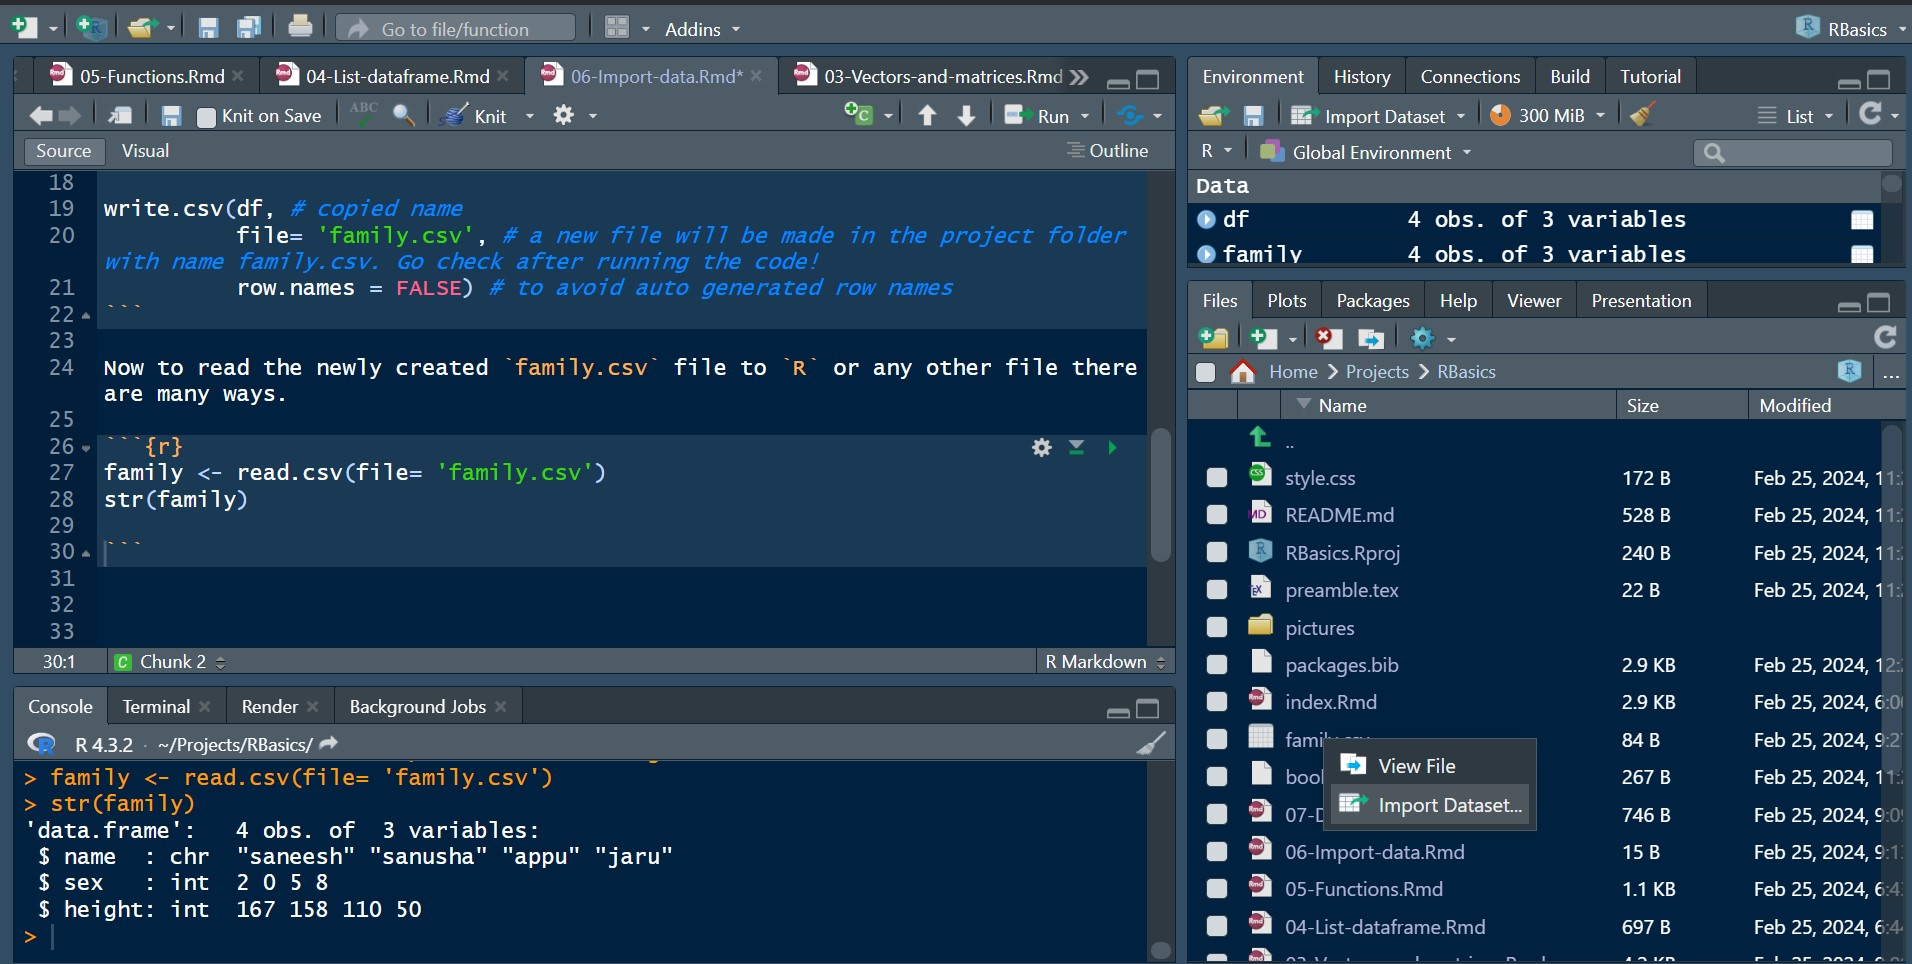
\includegraphics[width=1\linewidth]{pictures/importcsv} 

}

\caption{Files .csv file}\label{fig:unnamed-chunk-46}
\end{figure}

\begin{figure}

{\centering 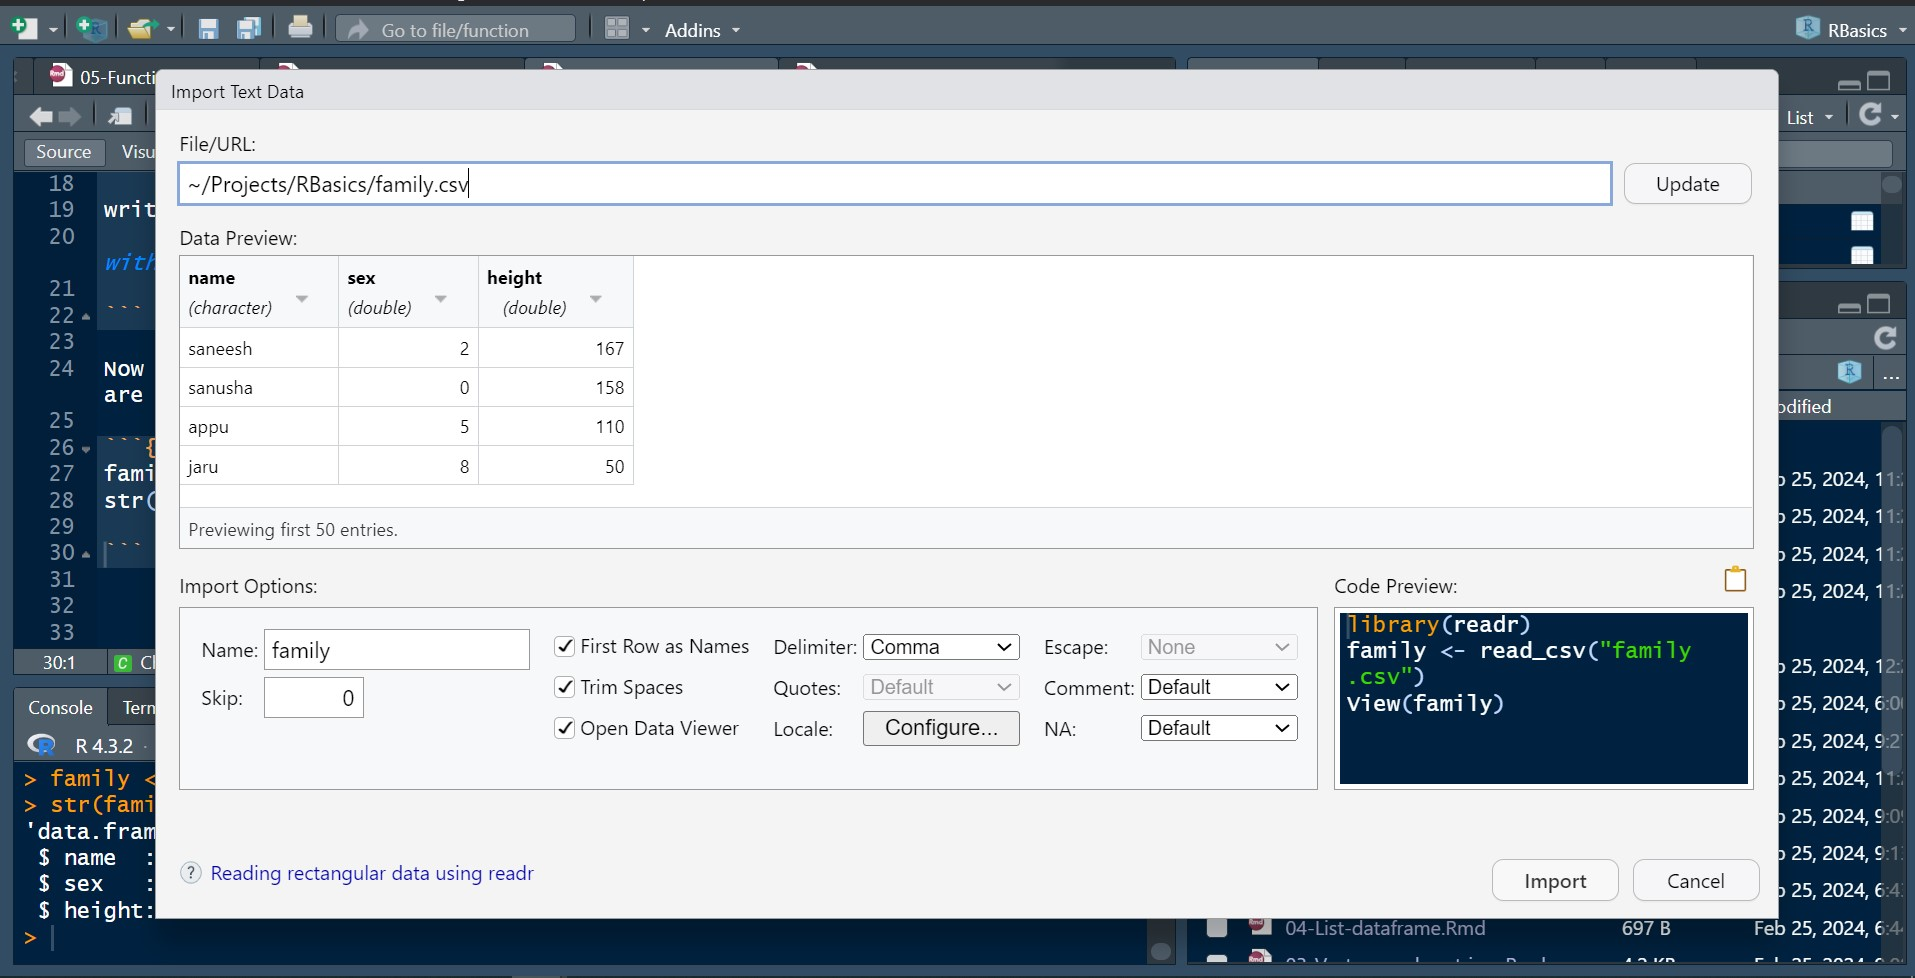
\includegraphics[width=1\linewidth]{pictures/importcsv_1} 

}

\caption{Files .csv file}\label{fig:unnamed-chunk-47}
\end{figure}

Look at the data preview, import options (change \texttt{Name} if needed), click \texttt{Import}. or copy code from \texttt{code\ preview}, click on \texttt{cancel} and paste the code on the script panel and \texttt{Run}. If you don't have \texttt{readr} package \texttt{R} will show an error, don't worry read the message and \texttt{install.packages(\textquotesingle{}readr\textquotesingle{})} will solve the problem, then run the code again.

\hypertarget{data-visualization}{%
\chapter{Data Visualization}\label{data-visualization}}

Condensing intricate data into numerical summaries inevitably leads to some loss of information. Visualization, though it also involves some information loss, can be less so when executed effectively. A thorough data analysis should always begin with a phase where the analyst deeply familiarizes themselves with the data they're working with. This process of gaining a deep understanding is integral to data analysis, and visualization plays a crucial role in it.

The vague \& defeasible rule of thumb of good data visualization (according to the Edward Tufte).

\begin{quote}
``Communicate a maximal degree of relevant true information in a way that minimizes the recipient's effort of retrieving this information.''
\end{quote}

\hypertarget{scatter-plot}{%
\section{Scatter plot}\label{scatter-plot}}

\texttt{?geom\_point}, try to to know more about geom\_points
The point geom is used to create scatterplots. The scatterplot is most useful for displaying the relationship between two continuous variables.

\hypertarget{let-us-make-some-data.}{%
\subsection{Let us make some data.}\label{let-us-make-some-data.}}

Imagine Shubham and I are planning to do a research on how Cashew and Teak respond to a new fertilizer we invented!!

To make the data we will use \texttt{ggplot2} and \texttt{dplyr}, we can use \texttt{tidyverse} so both packages will be loaded.

We also want to check if the trees in the fertilizer treatment can store more carbon. I don't know how scientifically correct this is but I am using this resource \href{https://naturalresources.wales/media/687190/eng-worksheet-carbon-storage-calculator.pdf}{Carbon storage calculator}. Based on this I wrote a function, read the \texttt{Chapter\ 6} for additional information on functions.

\hypertarget{carbon-calculator-function}{%
\subsection{carbon calculator function}\label{carbon-calculator-function}}

\begin{Shaded}
\begin{Highlighting}[]
\NormalTok{carbon\_calc }\OtherTok{\textless{}{-}} \ControlFlowTok{function}\NormalTok{(x) \{}
\NormalTok{  dry\_weight }\OtherTok{=}\NormalTok{ x }\SpecialCharTok{*} \FloatTok{13.0933}
\NormalTok{  carbon }\OtherTok{=} \FunctionTok{round}\NormalTok{(dry\_weight }\SpecialCharTok{/} \DecValTok{2}\NormalTok{)}
  \FunctionTok{return}\NormalTok{(carbon)}
\NormalTok{\}}

\FunctionTok{carbon\_calc}\NormalTok{(}\DecValTok{1}\NormalTok{)}
\end{Highlighting}
\end{Shaded}

\begin{verbatim}
## [1] 7
\end{verbatim}

\begin{Shaded}
\begin{Highlighting}[]
\CommentTok{\# treatment (factor)}
\FunctionTok{library}\NormalTok{(ggplot2)}
\FunctionTok{library}\NormalTok{(dplyr)}
\end{Highlighting}
\end{Shaded}

\begin{verbatim}
## 
## Attaching package: 'dplyr'
\end{verbatim}

\begin{verbatim}
## The following objects are masked from 'package:stats':
## 
##     filter, lag
\end{verbatim}

\begin{verbatim}
## The following objects are masked from 'package:base':
## 
##     intersect, setdiff, setequal, union
\end{verbatim}

\begin{Shaded}
\begin{Highlighting}[]
\CommentTok{\# new df with treatment}
\FunctionTok{set.seed}\NormalTok{(}\DecValTok{007}\NormalTok{) }\CommentTok{\# the name is Bond, James Bond= 007, its just a number. If you want the same result as mine use this set.seed number.}
\CommentTok{\# new df with treatment}

\NormalTok{treatment }\OtherTok{\textless{}{-}} \FunctionTok{c}\NormalTok{(}\FunctionTok{rep}\NormalTok{(}\StringTok{\textquotesingle{}nofertilizer\textquotesingle{}}\NormalTok{, }\DecValTok{50}\NormalTok{), }
               \FunctionTok{rep}\NormalTok{(}\StringTok{\textquotesingle{}fertilizer\textquotesingle{}}\NormalTok{, }\DecValTok{50}\NormalTok{))}

\NormalTok{name }\OtherTok{\textless{}{-}} \FunctionTok{c}\NormalTok{(}\FunctionTok{rep}\NormalTok{(}\StringTok{\textquotesingle{}cashew\textquotesingle{}}\NormalTok{, }\DecValTok{100}\NormalTok{), }
          \FunctionTok{rep}\NormalTok{(}\StringTok{\textquotesingle{}teak\textquotesingle{}}\NormalTok{, }\DecValTok{100}\NormalTok{))}

\NormalTok{gbh }\OtherTok{\textless{}{-}} \FunctionTok{c}\NormalTok{(}\FunctionTok{rnorm}\NormalTok{(}\DecValTok{50}\NormalTok{,}
             \AttributeTok{mean =} \DecValTok{15}\NormalTok{,}
             \AttributeTok{sd =} \DecValTok{4}\NormalTok{),}
         \FunctionTok{rnorm}\NormalTok{(}\DecValTok{50}\NormalTok{,}
               \AttributeTok{mean =} \DecValTok{30}\NormalTok{,}
               \AttributeTok{sd =} \DecValTok{6}\NormalTok{))}

\NormalTok{df }\OtherTok{\textless{}{-}} \FunctionTok{data.frame}\NormalTok{(treatment, }
\NormalTok{                 name, }
\NormalTok{                 gbh)}

\FunctionTok{str}\NormalTok{(df)}
\end{Highlighting}
\end{Shaded}

\begin{verbatim}
## 'data.frame':    200 obs. of  3 variables:
##  $ treatment: chr  "nofertilizer" "nofertilizer" "nofertilizer" "nofertilizer" ...
##  $ name     : chr  "cashew" "cashew" "cashew" "cashew" ...
##  $ gbh      : num  24.1 10.2 12.2 13.4 11.1 ...
\end{verbatim}

\begin{Shaded}
\begin{Highlighting}[]
\NormalTok{newdf }\OtherTok{\textless{}{-}}\NormalTok{ df }\SpecialCharTok{\%\textgreater{}\%} 
  \FunctionTok{filter}\NormalTok{(gbh  }\SpecialCharTok{\textgreater{}=} \DecValTok{15}\NormalTok{) }

\NormalTok{co }\OtherTok{\textless{}{-}} \FunctionTok{rnorm}\NormalTok{(}\FunctionTok{length}\NormalTok{(newdf}\SpecialCharTok{$}\NormalTok{gbh), }\FunctionTok{carbon\_calc}\NormalTok{(}\DecValTok{1}\NormalTok{), }\FloatTok{1.5}\NormalTok{) }\CommentTok{\# kg}

\NormalTok{newdf }\OtherTok{\textless{}{-}}\NormalTok{ newdf }\SpecialCharTok{\%\textgreater{}\%} 
  \FunctionTok{mutate}\NormalTok{(}\AttributeTok{co2=}\NormalTok{ gbh }\SpecialCharTok{*}\NormalTok{ co) }\CommentTok{\# co2 is a new column based gbh}

\FunctionTok{str}\NormalTok{(newdf)}
\end{Highlighting}
\end{Shaded}

\begin{verbatim}
## 'data.frame':    154 obs. of  4 variables:
##  $ treatment: chr  "nofertilizer" "nofertilizer" "nofertilizer" "nofertilizer" ...
##  $ name     : chr  "cashew" "cashew" "cashew" "cashew" ...
##  $ gbh      : num  24.1 18 15.6 23.8 16.4 ...
##  $ co2      : num  188 142 107 124 123 ...
\end{verbatim}

\begin{Shaded}
\begin{Highlighting}[]
\FunctionTok{names}\NormalTok{(newdf)}
\end{Highlighting}
\end{Shaded}

\begin{verbatim}
## [1] "treatment" "name"      "gbh"       "co2"
\end{verbatim}

\begin{Shaded}
\begin{Highlighting}[]
\FunctionTok{ggplot}\NormalTok{(}\AttributeTok{data =}\NormalTok{ newdf, }\FunctionTok{aes}\NormalTok{(}\AttributeTok{x =}\NormalTok{ gbh, }\AttributeTok{y =}\NormalTok{ co2, }\AttributeTok{col=}\NormalTok{ name)) }\SpecialCharTok{+}
  \FunctionTok{geom\_point}\NormalTok{() }\SpecialCharTok{+}
  \FunctionTok{geom\_smooth}\NormalTok{(}\AttributeTok{method =} \StringTok{\textquotesingle{}lm\textquotesingle{}}\NormalTok{) }\SpecialCharTok{+}
  \FunctionTok{facet\_wrap}\NormalTok{(}\SpecialCharTok{\textasciitilde{}}\NormalTok{ name)}
\end{Highlighting}
\end{Shaded}

\begin{verbatim}
## `geom_smooth()` using formula = 'y ~ x'
\end{verbatim}

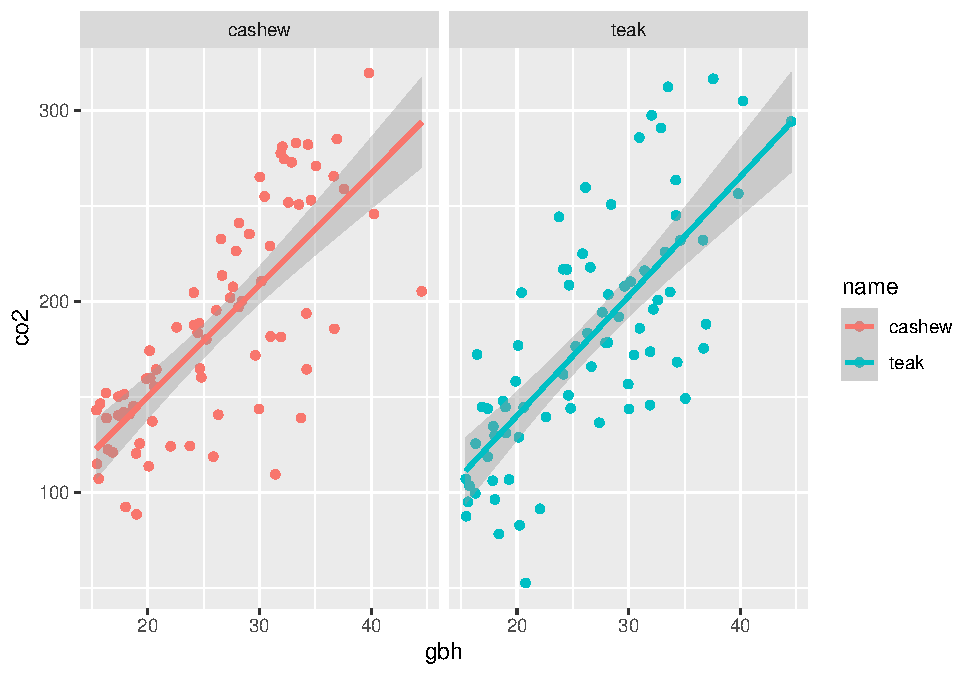
\includegraphics{_main_files/figure-latex/unnamed-chunk-49-1.pdf}

\begin{Shaded}
\begin{Highlighting}[]
\CommentTok{\# To know what facet\_wrap is}

\CommentTok{\# ?facet\_wrap}
\CommentTok{\# help(facet\_wrap)}
\end{Highlighting}
\end{Shaded}

\hypertarget{box-plot}{%
\section{Box plot}\label{box-plot}}

A box and whisker plot or diagram (otherwise known as a boxplot), is a graph summarising a set of data. The shape of the boxplot shows how the data is distributed and it also shows any \href{https://www.ncl.ac.uk/webtemplate/ask-assets/external/maths-resources/statistics/descriptive-statistics/other-measures-of-dispersion.html\#Outliers}{outliers}. It is a useful way to compare different sets of data as you can draw more than one boxplot per graph. These can be displayed alongside a number line, horizontally or vertically.\\
\emph{Reading a Box and Whisker Plot}\\
Interpreting a boxplot can be done once you understand what the different lines mean on a box and whisker diagram. The line splitting the box in two represents the median value. This shows that 50 \% of the data lies on the left hand side of the median value and 50 \% lies on the right hand side. The left edge of the box represents the lower \href{https://www.ncl.ac.uk/webtemplate/ask-assets/external/maths-resources/statistics/descriptive-statistics/other-measures-of-dispersion.html\#Quartiles}{quartile}; it shows the value at which the first 25 \% of the data falls up to. The right edge of the box shows the upper \href{https://www.ncl.ac.uk/webtemplate/ask-assets/external/maths-resources/statistics/descriptive-statistics/other-measures-of-dispersion.html\#Quartiles}{quartile}; it shows that 25 \% of the data lies to the right of the upper quartile value. The values at which the horizontal lines stop at are the values of the upper and lower values of the data. The single points on the diagram show the outliers.\\
\texttt{geom\_boxplot} function from \texttt{ggplot2} compactly displays the distribution of a continuous variable and a categorical variable, see Figure (Boxplot)

\begin{figure}

{\centering 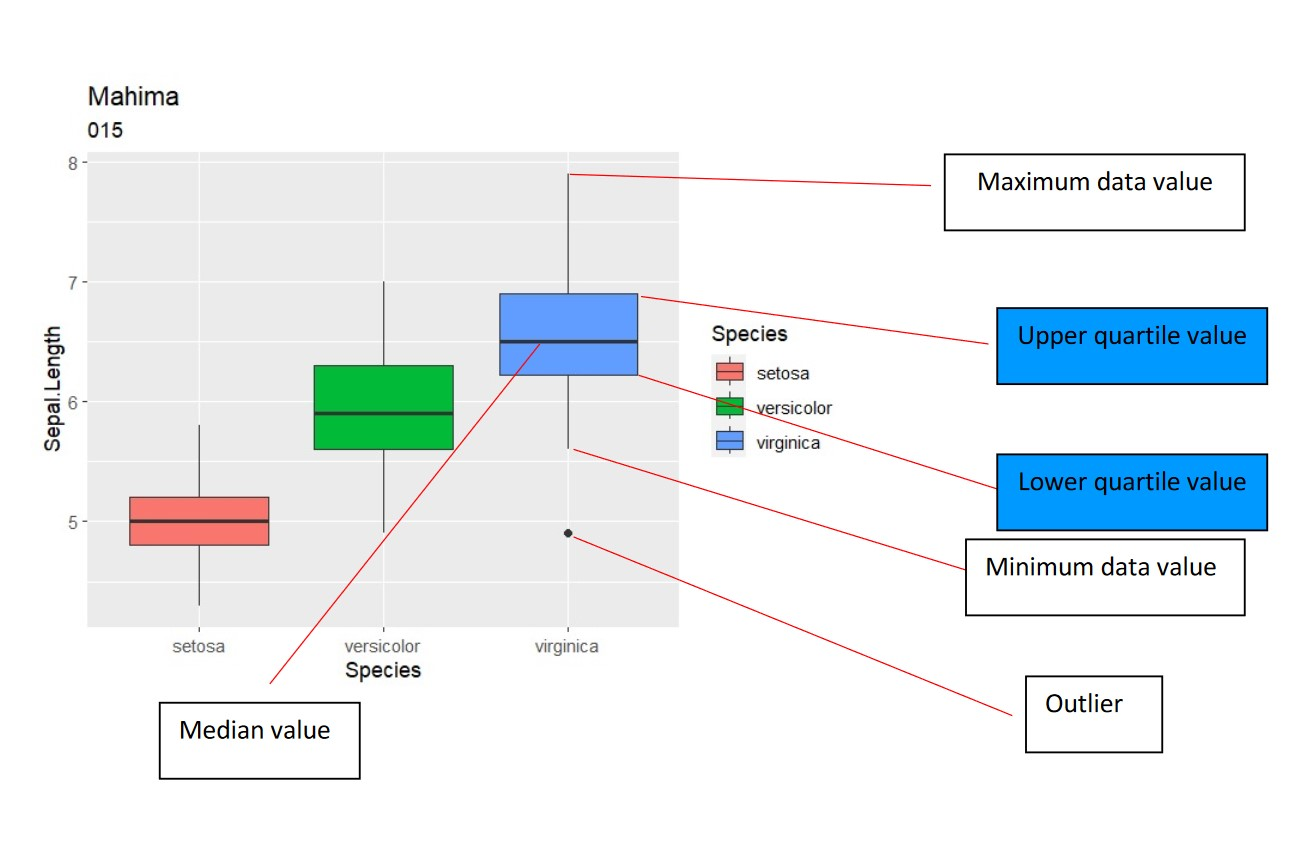
\includegraphics[width=1\linewidth]{pictures/boxplot} 

}

\caption{Boxplot}\label{fig:unnamed-chunk-50}
\end{figure}

\begin{Shaded}
\begin{Highlighting}[]
\FunctionTok{ggplot}\NormalTok{(}\AttributeTok{data =}\NormalTok{ newdf,}
       \FunctionTok{aes}\NormalTok{(}\AttributeTok{x =}\NormalTok{ treatment,}
           \AttributeTok{y =}\NormalTok{ co2,}
           \AttributeTok{fill =}\NormalTok{ name)) }\SpecialCharTok{+}
  \FunctionTok{geom\_boxplot}\NormalTok{() }\SpecialCharTok{+}
  \FunctionTok{facet\_wrap}\NormalTok{( }\SpecialCharTok{\textasciitilde{}}\NormalTok{ name)}
\end{Highlighting}
\end{Shaded}

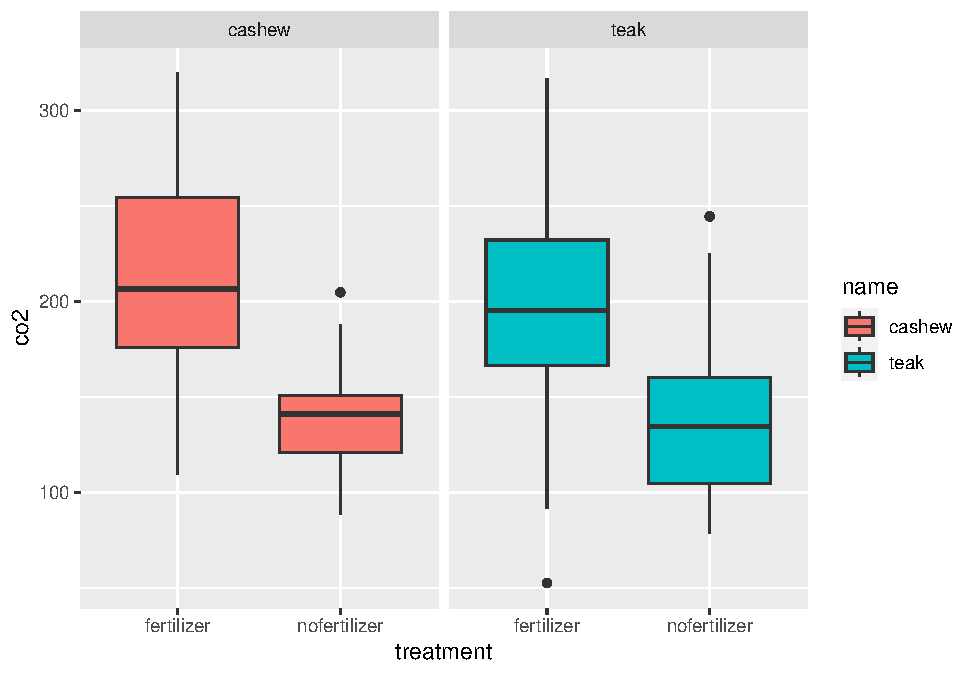
\includegraphics{_main_files/figure-latex/unnamed-chunk-51-1.pdf}

\begin{Shaded}
\begin{Highlighting}[]
\FunctionTok{ggplot}\NormalTok{(}\AttributeTok{data =}\NormalTok{ newdf,}
       \FunctionTok{aes}\NormalTok{(}\AttributeTok{y =}\NormalTok{ gbh,}
           \AttributeTok{x =}\NormalTok{ treatment,}
           \AttributeTok{fill =}\NormalTok{ name)) }\SpecialCharTok{+}
  \FunctionTok{geom\_boxplot}\NormalTok{()}
\end{Highlighting}
\end{Shaded}

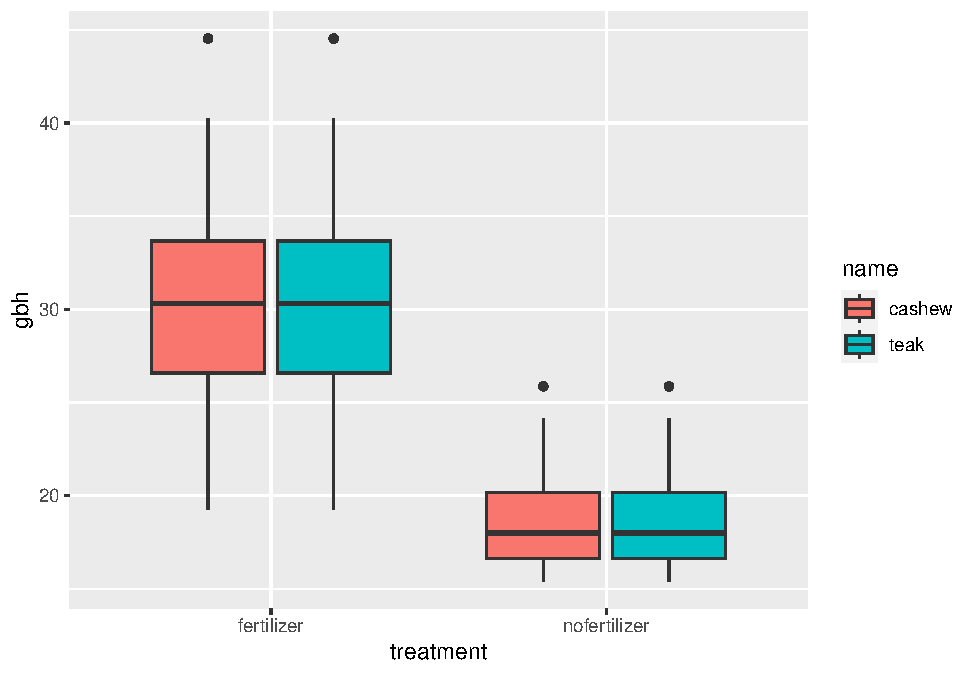
\includegraphics{_main_files/figure-latex/unnamed-chunk-51-2.pdf}

\hypertarget{wordcloud}{%
\chapter{Wordcloud}\label{wordcloud}}

\hypertarget{wordcloud-from-data-frame}{%
\section{Wordcloud from data frame}\label{wordcloud-from-data-frame}}

\begin{Shaded}
\begin{Highlighting}[]
\CommentTok{\# install.packages("dplyr")}
\CommentTok{\# install.packages(\textquotesingle{}wordcloud\textquotesingle{})}

\CommentTok{\# add packages{-}{-}{-}{-}}
\FunctionTok{library}\NormalTok{(dplyr) }\CommentTok{\# to clean data}
\FunctionTok{library}\NormalTok{(wordcloud) }\CommentTok{\# to make wordcloud}
\end{Highlighting}
\end{Shaded}

\begin{verbatim}
## Loading required package: RColorBrewer
\end{verbatim}

\hypertarget{read-data}{%
\subsection{Read data}\label{read-data}}

\begin{Shaded}
\begin{Highlighting}[]
\NormalTok{words }\OtherTok{\textless{}{-}} \FunctionTok{data.frame}\NormalTok{(}\AttributeTok{Name=} \FunctionTok{c}\NormalTok{(}\FunctionTok{rep}\NormalTok{(}\StringTok{\textquotesingle{}James Bond\textquotesingle{}}\NormalTok{, }\DecValTok{30}\NormalTok{),}
                    \FunctionTok{rep}\NormalTok{(}\StringTok{\textquotesingle{}Iron Man\textquotesingle{}}\NormalTok{, }\DecValTok{20}\NormalTok{),}
                    \FunctionTok{rep}\NormalTok{(}\StringTok{\textquotesingle{}Spider Man\textquotesingle{}}\NormalTok{, }\DecValTok{5}\NormalTok{),}
                    \FunctionTok{rep}\NormalTok{(}\StringTok{\textquotesingle{}Caption America\textquotesingle{}}\NormalTok{, }\DecValTok{4}\NormalTok{)),}
                    \AttributeTok{Tag=} \FunctionTok{c}\NormalTok{(}\FunctionTok{rep}\NormalTok{(}\StringTok{\textquotesingle{}Spy\textquotesingle{}}\NormalTok{, }\DecValTok{30}\NormalTok{),}
                               \FunctionTok{rep}\NormalTok{(}\StringTok{\textquotesingle{}Super hero\textquotesingle{}}\NormalTok{, }\DecValTok{29}\NormalTok{)),}
                    \AttributeTok{Duty=} \FunctionTok{c}\NormalTok{(}\FunctionTok{rep}\NormalTok{(}\StringTok{\textquotesingle{}kill\textquotesingle{}}\NormalTok{, }\DecValTok{30}\NormalTok{),}
                            \FunctionTok{rep}\NormalTok{(}\StringTok{\textquotesingle{}developer\textquotesingle{}}\NormalTok{, }\DecValTok{20}\NormalTok{),}
                            \FunctionTok{rep}\NormalTok{(}\StringTok{\textquotesingle{}save\textquotesingle{}}\NormalTok{, }\DecValTok{5}\NormalTok{),}
                            \FunctionTok{rep}\NormalTok{(}\StringTok{\textquotesingle{}save\textquotesingle{}}\NormalTok{, }\DecValTok{4}\NormalTok{)))}

\FunctionTok{str}\NormalTok{(words) }\CommentTok{\# display the internal structure \textasciigrave{}object\textasciigrave{}, here, our \textasciigrave{}data\textasciigrave{}}
\end{Highlighting}
\end{Shaded}

\begin{verbatim}
## 'data.frame':    59 obs. of  3 variables:
##  $ Name: chr  "James Bond" "James Bond" "James Bond" "James Bond" ...
##  $ Tag : chr  "Spy" "Spy" "Spy" "Spy" ...
##  $ Duty: chr  "kill" "kill" "kill" "kill" ...
\end{verbatim}

\begin{Shaded}
\begin{Highlighting}[]
\FunctionTok{head}\NormalTok{(words, }\DecValTok{3}\NormalTok{) }\CommentTok{\# change the number in the () and see more rows}
\end{Highlighting}
\end{Shaded}

\begin{verbatim}
##         Name Tag Duty
## 1 James Bond Spy kill
## 2 James Bond Spy kill
## 3 James Bond Spy kill
\end{verbatim}

\begin{Shaded}
\begin{Highlighting}[]
\FunctionTok{tail}\NormalTok{(words, }\DecValTok{3}\NormalTok{)}
\end{Highlighting}
\end{Shaded}

\begin{verbatim}
##               Name        Tag Duty
## 57 Caption America Super hero save
## 58 Caption America Super hero save
## 59 Caption America Super hero save
\end{verbatim}

\begin{Shaded}
\begin{Highlighting}[]
\CommentTok{\# let us see what is the duty of our heros}
\FunctionTok{names}\NormalTok{(words) }\CommentTok{\# to see the column names of words}
\end{Highlighting}
\end{Shaded}

\begin{verbatim}
## [1] "Name" "Tag"  "Duty"
\end{verbatim}

\begin{Shaded}
\begin{Highlighting}[]
\CommentTok{\# to add count to the data}
\NormalTok{words1 }\OtherTok{\textless{}{-}}\NormalTok{ words }\SpecialCharTok{\%\textgreater{}\%} \FunctionTok{count}\NormalTok{(Duty) }\CommentTok{\# words1 is a new data frame we created from words}
\end{Highlighting}
\end{Shaded}

\begin{Shaded}
\begin{Highlighting}[]
\FunctionTok{names}\NormalTok{(words1)}
\end{Highlighting}
\end{Shaded}

\begin{verbatim}
## [1] "Duty" "n"
\end{verbatim}

\begin{Shaded}
\begin{Highlighting}[]
\FunctionTok{max}\NormalTok{(words1}\SpecialCharTok{$}\NormalTok{n) }\CommentTok{\# copy this number for max.words=}
\end{Highlighting}
\end{Shaded}

\begin{verbatim}
## [1] 30
\end{verbatim}

\begin{Shaded}
\begin{Highlighting}[]
\CommentTok{\# par(bg="black") \# for black background}
\end{Highlighting}
\end{Shaded}

Before you plot, make sure that the \texttt{Files}, \texttt{Plot} \texttt{Packages} panel is maximized!! click on the rectangular button on top of the File, Plots, Packages window.

\begin{Shaded}
\begin{Highlighting}[]
\FunctionTok{wordcloud}\NormalTok{(}\AttributeTok{word =}\NormalTok{ words1}\SpecialCharTok{$}\NormalTok{Duty, }\CommentTok{\# BroaderGoal from the words1}
          \AttributeTok{freq =}\NormalTok{ words1}\SpecialCharTok{$}\NormalTok{n, }\CommentTok{\# n from the words1 data frame}
          \AttributeTok{min.freq =} \DecValTok{1}\NormalTok{, }\CommentTok{\# minimum frequency of a word}
          \AttributeTok{max.words =} \DecValTok{14}\NormalTok{, }\CommentTok{\# maximum frequency of a word}
          \AttributeTok{random.order=}\NormalTok{T,}
          \CommentTok{\# colors = brewer.pal(6, \textquotesingle{}GnBu\textquotesingle{}) \# remove comment from}
          \CommentTok{\# these code one by one and see how color change}
          \CommentTok{\# colors = brewer.pal(6, \textquotesingle{}Reds\textquotesingle{})}
          \CommentTok{\# colors = brewer.pal(6, \textquotesingle{}Blues\textquotesingle{})}
          \CommentTok{\# colors = brewer.pal(1, \textquotesingle{}Reds\textquotesingle{})}
          \AttributeTok{colors=}\FunctionTok{brewer.pal}\NormalTok{(}\DecValTok{8}\NormalTok{, }\StringTok{"Dark2"}\NormalTok{)}
\NormalTok{          )}
\end{Highlighting}
\end{Shaded}


\includegraphics{_main_files/figure-latex/unnamed-chunk-56-1.pdf}

Let us see what are they known as

\begin{Shaded}
\begin{Highlighting}[]
\FunctionTok{names}\NormalTok{(words) }\CommentTok{\# to see the column names of words}
\end{Highlighting}
\end{Shaded}

\begin{verbatim}
## [1] "Name" "Tag"  "Duty"
\end{verbatim}

\begin{Shaded}
\begin{Highlighting}[]
\CommentTok{\# know the data}
\NormalTok{words2 }\OtherTok{\textless{}{-}}\NormalTok{ words }\SpecialCharTok{\%\textgreater{}\%} \FunctionTok{count}\NormalTok{(Tag)}

\FunctionTok{names}\NormalTok{(words2)}
\end{Highlighting}
\end{Shaded}

\begin{verbatim}
## [1] "Tag" "n"
\end{verbatim}

\begin{Shaded}
\begin{Highlighting}[]
\FunctionTok{max}\NormalTok{(words2}\SpecialCharTok{$}\NormalTok{n) }\CommentTok{\# copy this number for max.words=}
\end{Highlighting}
\end{Shaded}

\begin{verbatim}
## [1] 30
\end{verbatim}

Before you plot, make sure that the plot window or Plot pane is maximized!! click on the rectangular button on top of the \texttt{File}, \texttt{Plots}, \texttt{Packages} window.

\begin{Shaded}
\begin{Highlighting}[]
\CommentTok{\# par(bg="black") \# for black background}

\FunctionTok{wordcloud}\NormalTok{(}\AttributeTok{word =}\NormalTok{ words2}\SpecialCharTok{$}\NormalTok{Tag, }\CommentTok{\# BroderBackground from the words2}
          \AttributeTok{freq =}\NormalTok{ words2}\SpecialCharTok{$}\NormalTok{n, }\CommentTok{\# n from the words2 data frame}
          \AttributeTok{min.freq =} \DecValTok{1}\NormalTok{, }\CommentTok{\# minimum frequency of a word}
          \AttributeTok{max.words =} \DecValTok{10}\NormalTok{, }\CommentTok{\# maximum frequency of a word}
          \AttributeTok{random.order=}\NormalTok{T,}
          \CommentTok{\# vfont= c(family= \textquotesingle{}gothic english\textquotesingle{}, face= \textquotesingle{}plain\textquotesingle{}), \# fonts, remove comment from}
          \CommentTok{\# these code one by one and see how font and color change}
          \CommentTok{\# vfont= c(family= \textquotesingle{}script\textquotesingle{}, face= \textquotesingle{}plain\textquotesingle{}),}
          \CommentTok{\# vfont= c(family= \textquotesingle{}serif\textquotesingle{}, face= \textquotesingle{}plain\textquotesingle{}),}
          \CommentTok{\# vfont= c(family= \textquotesingle{}sans serif\textquotesingle{}, face= \textquotesingle{}plain\textquotesingle{}),}
          \AttributeTok{vfont=} \FunctionTok{c}\NormalTok{(}\AttributeTok{family=} \StringTok{\textquotesingle{}serif\textquotesingle{}}\NormalTok{, }\AttributeTok{face=} \StringTok{\textquotesingle{}cyrillic\textquotesingle{}}\NormalTok{),}
          \CommentTok{\# colors = brewer.pal(6, \textquotesingle{}GnBu\textquotesingle{}) \# colors}
          \AttributeTok{colors =} \FunctionTok{brewer.pal}\NormalTok{(}\DecValTok{6}\NormalTok{, }\StringTok{\textquotesingle{}Reds\textquotesingle{}}\NormalTok{)}
          \CommentTok{\# colors = brewer.pal(6, \textquotesingle{}Blues\textquotesingle{})}
          \CommentTok{\# colors = brewer.pal(1, \textquotesingle{}Reds\textquotesingle{})}
          \CommentTok{\# colors=brewer.pal(8, "Dark2")}
\NormalTok{)}
\end{Highlighting}
\end{Shaded}


\includegraphics{_main_files/figure-latex/unnamed-chunk-58-1.pdf}

If the plot doesn't look good restart R from Session tab or press Ctrl+Shift+F10, then start from add packages :). If you want to change background bg= ``black'' or other colors do the above, restart. If you are happy with a plot, Export\textgreater{} Save as PDF\textgreater{} select PDF Size\textgreater{} change directory if you want.

\hypertarget{wordcloud-from-text-data}{%
\section{Wordcloud from text data}\label{wordcloud-from-text-data}}

\begin{Shaded}
\begin{Highlighting}[]
\CommentTok{\# packages{-}{-}{-}{-}}
\CommentTok{\# install.packages(\textquotesingle{}tm\textquotesingle{})}
\CommentTok{\# install.packages(\textquotesingle{}wordcloud\textquotesingle{})}
\end{Highlighting}
\end{Shaded}

Load packages

\begin{Shaded}
\begin{Highlighting}[]
\FunctionTok{library}\NormalTok{(tm)}
\end{Highlighting}
\end{Shaded}

\begin{verbatim}
## Loading required package: NLP
\end{verbatim}

\begin{verbatim}
## 
## Attaching package: 'NLP'
\end{verbatim}

\begin{verbatim}
## The following object is masked from 'package:ggplot2':
## 
##     annotate
\end{verbatim}

\begin{Shaded}
\begin{Highlighting}[]
\FunctionTok{library}\NormalTok{(wordcloud)}
\end{Highlighting}
\end{Shaded}

Text

\begin{Shaded}
\begin{Highlighting}[]
\NormalTok{mytext }\OtherTok{\textless{}{-}} \StringTok{"India, a vibrant land where ancient traditions dance with modern aspirations, pulsates with the rhythm of diversity. Its people, a kaleidoscope of ethnicities, languages, and religions, paint a masterpiece of cultural richness. From the snow{-}capped peaks of the Himalayas to the sun{-}drenched beaches of Goa, India\textquotesingle{}s diversity unfolds in every corner. In bustling metropolises like Mumbai and Delhi, the aroma of spices mingles with the scent of incense, each street alive with the echoes of diverse laughter and prayers. Travel south, and serene temple bells chime in Kerala, their melodies intertwining with the rhythmic beats of Kathakali dancers. Journey east, and the vibrant hues of sarees in Assam blend seamlessly with the bamboo houses of tribal communities. Every region in India whispers its own unique story, its people celebrating their distinct cultures with festivals like Holi, Diwali, and Onam, each a vibrant explosion of colors and traditions. The spirit of India lies in its diversity, a vibrant tapestry woven with countless threads of languages, customs, and beliefs.It is a land where unity thrives amidst difference, where the warmth of its people embraces every visitor, inviting them to experience the magic of its kaleidoscope soul. So, come, explore the diversity of India, and discover a land that will forever captivate your heart."} \CommentTok{\# inside the " "}
\end{Highlighting}
\end{Shaded}

\begin{Shaded}
\begin{Highlighting}[]
\NormalTok{mycorpus }\OtherTok{\textless{}{-}} \FunctionTok{Corpus}\NormalTok{(}\FunctionTok{VectorSource}\NormalTok{(mytext))}

\NormalTok{mycorpus }\OtherTok{\textless{}{-}} \FunctionTok{tm\_map}\NormalTok{(mycorpus, removePunctuation)}
\end{Highlighting}
\end{Shaded}

\begin{verbatim}
## Warning in tm_map.SimpleCorpus(mycorpus, removePunctuation): transformation
## drops documents
\end{verbatim}

\begin{Shaded}
\begin{Highlighting}[]
\NormalTok{mycorpus }\OtherTok{\textless{}{-}} \FunctionTok{tm\_map}\NormalTok{(mycorpus, removeNumbers)}
\end{Highlighting}
\end{Shaded}

\begin{verbatim}
## Warning in tm_map.SimpleCorpus(mycorpus, removeNumbers): transformation drops
## documents
\end{verbatim}

\begin{Shaded}
\begin{Highlighting}[]
\NormalTok{mycorpus }\OtherTok{\textless{}{-}} \FunctionTok{tm\_map}\NormalTok{(mycorpus, removeWords, }\FunctionTok{stopwords}\NormalTok{(}\StringTok{"english"}\NormalTok{))}
\end{Highlighting}
\end{Shaded}

\begin{verbatim}
## Warning in tm_map.SimpleCorpus(mycorpus, removeWords, stopwords("english")):
## transformation drops documents
\end{verbatim}

\begin{Shaded}
\begin{Highlighting}[]
\NormalTok{mywords }\OtherTok{\textless{}{-}} \FunctionTok{TermDocumentMatrix}\NormalTok{(mycorpus)}
\NormalTok{m }\OtherTok{\textless{}{-}} \FunctionTok{as.matrix}\NormalTok{(mywords)}
\NormalTok{v }\OtherTok{\textless{}{-}} \FunctionTok{sort}\NormalTok{(}\FunctionTok{rowSums}\NormalTok{(m), }\AttributeTok{decreasing=}\ConstantTok{TRUE}\NormalTok{)}

\CommentTok{\#make wordcloud{-}{-}{-}{-}}
\FunctionTok{wordcloud}\NormalTok{(}\FunctionTok{names}\NormalTok{(v), v, }\AttributeTok{scale=}\FunctionTok{c}\NormalTok{(}\DecValTok{3}\NormalTok{,}\FloatTok{0.5}\NormalTok{), }\AttributeTok{min.freq =} \DecValTok{1}\NormalTok{,}
          \AttributeTok{max.words=}\DecValTok{10}\NormalTok{, }\AttributeTok{random.order=}\ConstantTok{FALSE}\NormalTok{, }\AttributeTok{rot.per=}\FloatTok{0.35}\NormalTok{, }
          \AttributeTok{colors=}\FunctionTok{brewer.pal}\NormalTok{(}\DecValTok{8}\NormalTok{, }\StringTok{"Dark2"}\NormalTok{))}
\end{Highlighting}
\end{Shaded}

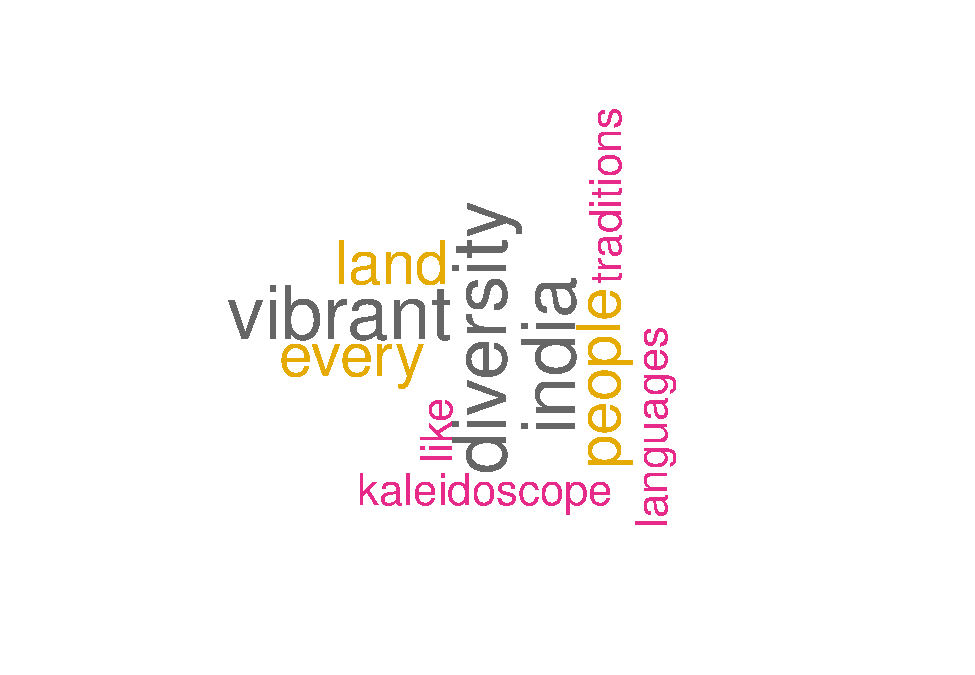
\includegraphics{_main_files/figure-latex/unnamed-chunk-62-1.pdf}

\begin{Shaded}
\begin{Highlighting}[]
\CommentTok{\# a word cloud for Indian budget}
\FunctionTok{library}\NormalTok{(rvest)}
\end{Highlighting}
\end{Shaded}

\begin{verbatim}
## 
## Attaching package: 'rvest'
\end{verbatim}

\begin{verbatim}
## The following object is masked from 'package:readr':
## 
##     guess_encoding
\end{verbatim}

\begin{Shaded}
\begin{Highlighting}[]
\FunctionTok{library}\NormalTok{(wordcloud)}
\FunctionTok{library}\NormalTok{(tm)}
\FunctionTok{library}\NormalTok{(Rgraphviz)}
\end{Highlighting}
\end{Shaded}

\begin{verbatim}
## Loading required package: graph
\end{verbatim}

\begin{verbatim}
## Loading required package: BiocGenerics
\end{verbatim}

\begin{verbatim}
## 
## Attaching package: 'BiocGenerics'
\end{verbatim}

\begin{verbatim}
## The following object is masked from 'package:NLP':
## 
##     annotation
\end{verbatim}

\begin{verbatim}
## The following objects are masked from 'package:dplyr':
## 
##     combine, intersect, setdiff, union
\end{verbatim}

\begin{verbatim}
## The following objects are masked from 'package:stats':
## 
##     IQR, mad, sd, var, xtabs
\end{verbatim}

\begin{verbatim}
## The following objects are masked from 'package:base':
## 
##     anyDuplicated, aperm, append, as.data.frame, basename, cbind,
##     colnames, dirname, do.call, duplicated, eval, evalq, Filter, Find,
##     get, grep, grepl, intersect, is.unsorted, lapply, Map, mapply,
##     match, mget, order, paste, pmax, pmax.int, pmin, pmin.int,
##     Position, rank, rbind, Reduce, rownames, sapply, setdiff, sort,
##     table, tapply, union, unique, unsplit, which.max, which.min
\end{verbatim}

\begin{verbatim}
## Loading required package: grid
\end{verbatim}

\begin{Shaded}
\begin{Highlighting}[]
\CommentTok{\# install.packages("BiocManager")}
\CommentTok{\# BiocManager::install("Rgraphviz")}


\CommentTok{\# budget}
\CommentTok{\# set path to the textfile}
\NormalTok{budget }\OtherTok{\textless{}{-}} \FunctionTok{read.delim}\NormalTok{(}\StringTok{\textquotesingle{}budget\_speech.txt\textquotesingle{}}\NormalTok{, }\AttributeTok{fileEncoding=}\StringTok{"UCS{-}2LE"}\NormalTok{)}
\end{Highlighting}
\end{Shaded}

\begin{verbatim}
## Warning in read.table(file = file, header = header, sep = sep, quote = quote, :
## incomplete final line found by readTableHeader on 'budget_speech.txt'
\end{verbatim}

\begin{Shaded}
\begin{Highlighting}[]
\CommentTok{\# Remove punctuation and numbers}
\NormalTok{budget }\OtherTok{\textless{}{-}} \FunctionTok{gsub}\NormalTok{(}\StringTok{"[[:punct:]0{-}9]"}\NormalTok{, }\StringTok{""}\NormalTok{, budget, }\AttributeTok{useBytes =} \ConstantTok{TRUE}\NormalTok{)}

\CommentTok{\# covert text to lowercase}
\NormalTok{budget }\OtherTok{\textless{}{-}} \FunctionTok{tolower}\NormalTok{(budget)}

\CommentTok{\# remove stopwords}
\NormalTok{stopwords }\OtherTok{\textless{}{-}} \FunctionTok{stopwords}\NormalTok{(}\StringTok{\textquotesingle{}SMART\textquotesingle{}}\NormalTok{) }\CommentTok{\# options \textquotesingle{}english\textquotesingle{}}

\NormalTok{budget }\OtherTok{\textless{}{-}}\NormalTok{ budget[}\SpecialCharTok{!}\NormalTok{budget }\SpecialCharTok{\%in\%}\NormalTok{ stopwords]}



\CommentTok{\# Create a corpus from the text}
\NormalTok{corpus }\OtherTok{\textless{}{-}} \FunctionTok{Corpus}\NormalTok{(}\FunctionTok{VectorSource}\NormalTok{(budget))}

\CommentTok{\# Create a term{-}document matrix}
\NormalTok{tdm }\OtherTok{\textless{}{-}} \FunctionTok{TermDocumentMatrix}\NormalTok{(corpus)}

\CommentTok{\# Convert the tdm to a matrix and calculate word frequencies}
\NormalTok{matr }\OtherTok{\textless{}{-}} \FunctionTok{as.matrix}\NormalTok{(tdm)}
\NormalTok{word\_freq }\OtherTok{\textless{}{-}} \FunctionTok{sort}\NormalTok{(}\FunctionTok{rowSums}\NormalTok{(matr), }\AttributeTok{decreasing =} \ConstantTok{TRUE}\NormalTok{)}
\end{Highlighting}
\end{Shaded}

\begin{Shaded}
\begin{Highlighting}[]
\FunctionTok{wordcloud}\NormalTok{(}\FunctionTok{names}\NormalTok{(word\_freq), }
\NormalTok{          word\_freq, }\AttributeTok{max.words =} \DecValTok{50}\NormalTok{, }\CommentTok{\# can change number of words }
          \AttributeTok{random.order =} \ConstantTok{FALSE}\NormalTok{, }
          \AttributeTok{colors =} \FunctionTok{brewer.pal}\NormalTok{(}\DecValTok{8}\NormalTok{, }\StringTok{"Dark2"}\NormalTok{))}
\end{Highlighting}
\end{Shaded}

It will look something like this!

\begin{figure}

{\centering 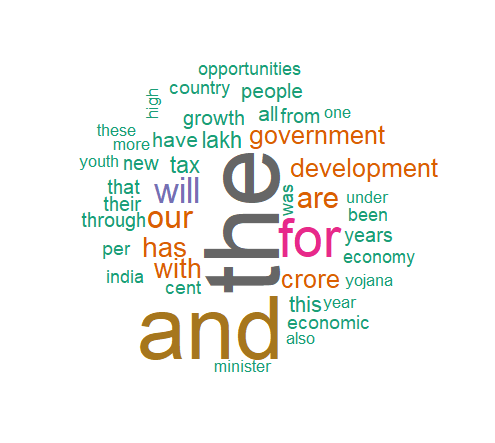
\includegraphics[width=1\linewidth]{pictures/budget_Speech} 

}

\caption{Budget word cloud}\label{fig:unnamed-chunk-64}
\end{figure}

\hypertarget{probability}{%
\chapter{Probability}\label{probability}}

\begin{Shaded}
\begin{Highlighting}[]
\FunctionTok{library}\NormalTok{(}\StringTok{\textquotesingle{}dplyr\textquotesingle{}}\NormalTok{, }\StringTok{\textquotesingle{}ggplot2\textquotesingle{}}\NormalTok{)}
\end{Highlighting}
\end{Shaded}

\begin{Shaded}
\begin{Highlighting}[]
\FunctionTok{set.seed}\NormalTok{(}\DecValTok{007}\NormalTok{) }\CommentTok{\# to ensure that the random sampling results are reproducible.}
\end{Highlighting}
\end{Shaded}

\hypertarget{create-vectors}{%
\section{create vectors}\label{create-vectors}}

\begin{Shaded}
\begin{Highlighting}[]
\NormalTok{species}\OtherTok{=} \FunctionTok{c}\NormalTok{(}\StringTok{\textquotesingle{}Tiger\textquotesingle{}}\NormalTok{, }\StringTok{\textquotesingle{}Deer\textquotesingle{}}\NormalTok{, }\StringTok{\textquotesingle{}Leopard\textquotesingle{}}\NormalTok{)}
\NormalTok{tiger\_reserve }\OtherTok{=} \FunctionTok{c}\NormalTok{(}\StringTok{\textquotesingle{}Kanha\textquotesingle{}}\NormalTok{, }\StringTok{\textquotesingle{}Bandipur\textquotesingle{}}\NormalTok{)}
\NormalTok{sighting }\OtherTok{=} \FunctionTok{c}\NormalTok{(}\DecValTok{1}\NormalTok{, }\DecValTok{0}\NormalTok{) }\CommentTok{\# 1 (for sighting) and 0 (for no sighting)}
\end{Highlighting}
\end{Shaded}

\hypertarget{make-a-data-frame-name-it-i-gave-df-data-frame}{%
\section{make a data frame, name it I gave df= data frame}\label{make-a-data-frame-name-it-i-gave-df-data-frame}}

\begin{Shaded}
\begin{Highlighting}[]
\NormalTok{df }\OtherTok{\textless{}{-}} \FunctionTok{data.frame}\NormalTok{(}
  \AttributeTok{species=} \FunctionTok{sample}\NormalTok{(}\AttributeTok{x =}\NormalTok{ species, }\DecValTok{20}\NormalTok{, }\AttributeTok{replace =}\NormalTok{ T), }\CommentTok{\# replace= T, for repeated sampling (with replacement)}
  \AttributeTok{tiger\_reserve=} \FunctionTok{sample}\NormalTok{(}\AttributeTok{x =}\NormalTok{ tiger\_reserve, }\DecValTok{20}\NormalTok{, }\AttributeTok{replace =}\NormalTok{ T),}
  \AttributeTok{sighting=} \FunctionTok{sample}\NormalTok{(}\AttributeTok{x =}\NormalTok{ sighting, }\DecValTok{20}\NormalTok{, }\AttributeTok{replace =}\NormalTok{ T)}
\NormalTok{)}
\end{Highlighting}
\end{Shaded}

\begin{Shaded}
\begin{Highlighting}[]
\FunctionTok{print}\NormalTok{(df)}
\end{Highlighting}
\end{Shaded}

\begin{verbatim}
##    species tiger_reserve sighting
## 1     Deer         Kanha        1
## 2  Leopard      Bandipur        0
## 3  Leopard         Kanha        1
## 4  Leopard      Bandipur        1
## 5     Deer      Bandipur        0
## 6  Leopard         Kanha        0
## 7     Deer      Bandipur        1
## 8     Deer      Bandipur        1
## 9  Leopard      Bandipur        1
## 10    Deer      Bandipur        1
## 11 Leopard         Kanha        0
## 12 Leopard      Bandipur        0
## 13    Deer      Bandipur        0
## 14 Leopard         Kanha        1
## 15    Deer         Kanha        0
## 16 Leopard      Bandipur        0
## 17 Leopard      Bandipur        1
## 18    Deer         Kanha        0
## 19    Deer         Kanha        0
## 20 Leopard         Kanha        0
\end{verbatim}

\hypertarget{calculating-total-sightings}{%
\section{calculating total sightings}\label{calculating-total-sightings}}

\begin{Shaded}
\begin{Highlighting}[]
\NormalTok{sightings\_total }\OtherTok{\textless{}{-}}\NormalTok{ df }\SpecialCharTok{\%\textgreater{}\%}
  \FunctionTok{group\_by}\NormalTok{(species, tiger\_reserve) }\SpecialCharTok{\%\textgreater{}\%}
  \FunctionTok{summarize}\NormalTok{(}\AttributeTok{total\_sightings =} \FunctionTok{sum}\NormalTok{(sighting))}
\end{Highlighting}
\end{Shaded}

\begin{verbatim}
## `summarise()` has grouped output by 'species'. You can override using the
## `.groups` argument.
\end{verbatim}

\hypertarget{calculate-the-probability-of-seeing-each-species}{%
\section{Calculate the probability of seeing each species}\label{calculate-the-probability-of-seeing-each-species}}

\begin{Shaded}
\begin{Highlighting}[]
\NormalTok{probabilities }\OtherTok{\textless{}{-}}\NormalTok{ sightings\_total }\SpecialCharTok{\%\textgreater{}\%}
  \FunctionTok{mutate}\NormalTok{ (}\AttributeTok{probability =}\NormalTok{ total\_sightings }\SpecialCharTok{/} \FunctionTok{sum}\NormalTok{(total\_sightings)) }\SpecialCharTok{\%\textgreater{}\%} 
  \FunctionTok{mutate}\NormalTok{ (}\AttributeTok{percentage =}\NormalTok{ probability}\SpecialCharTok{*}\DecValTok{100}\NormalTok{)}
\end{Highlighting}
\end{Shaded}

\begin{Shaded}
\begin{Highlighting}[]
\FunctionTok{library}\NormalTok{(report)}
\FunctionTok{print}\NormalTok{(probabilities)}
\end{Highlighting}
\end{Shaded}

\begin{verbatim}
## # A tibble: 4 x 5
## # Groups:   species [2]
##   species tiger_reserve total_sightings probability percentage
##   <chr>   <chr>                   <dbl>       <dbl>      <dbl>
## 1 Deer    Bandipur                    3        0.75         75
## 2 Deer    Kanha                       1        0.25         25
## 3 Leopard Bandipur                    3        0.6          60
## 4 Leopard Kanha                       2        0.4          40
\end{verbatim}

\begin{Shaded}
\begin{Highlighting}[]
\NormalTok{report}\SpecialCharTok{::}\FunctionTok{report\_statistics}\NormalTok{(probabilities)}
\end{Highlighting}
\end{Shaded}

\begin{verbatim}
## Deer, Bandipur, n = 1; Kanha, n = 1
## Deer, n = 2, Mean = 2.00, SD = 1.41, Median = 2.00, MAD = 1.48, range: [1, 3], Skewness = 0.00, Kurtosis = -2.00, 0 missing
## Deer, n = 2, Mean = 0.50, SD = 0.35, Median = 0.50, MAD = 0.37, range: [0.25, 0.75], Skewness = 0.00, Kurtosis = -2.00, 0 missing
## Deer, n = 2, Mean = 50.00, SD = 35.36, Median = 50.00, MAD = 37.06, range: [25, 75], Skewness = 0.00, Kurtosis = -2.00, 0 missing
## Leopard, Bandipur, n = 1; Kanha, n = 1
## Leopard, n = 2, Mean = 2.50, SD = 0.71, Median = 2.50, MAD = 0.74, range: [2, 3], Skewness = 0.00, Kurtosis = -2.00, 0 missing
## Leopard, n = 2, Mean = 0.50, SD = 0.14, Median = 0.50, MAD = 0.15, range: [0.40, 0.60], Skewness = 0.00, Kurtosis = -2.00, 0 missing
## Leopard, n = 2, Mean = 50.00, SD = 14.14, Median = 50.00, MAD = 14.83, range: [40, 60], Skewness = 0.00, Kurtosis = -2.00, 0 missing
\end{verbatim}

\begin{Shaded}
\begin{Highlighting}[]
\NormalTok{probabilities }\SpecialCharTok{\%\textgreater{}\%} \FunctionTok{ggplot}\NormalTok{(}\FunctionTok{aes}\NormalTok{(}\AttributeTok{x=}\NormalTok{ species, }\AttributeTok{y=}\NormalTok{ probability, }\AttributeTok{fill=}\NormalTok{ tiger\_reserve))}\SpecialCharTok{+}
  \FunctionTok{geom\_bar}\NormalTok{(}\AttributeTok{stat =} \StringTok{\textquotesingle{}identity\textquotesingle{}}\NormalTok{)}
\end{Highlighting}
\end{Shaded}

\begin{figure}
\centering
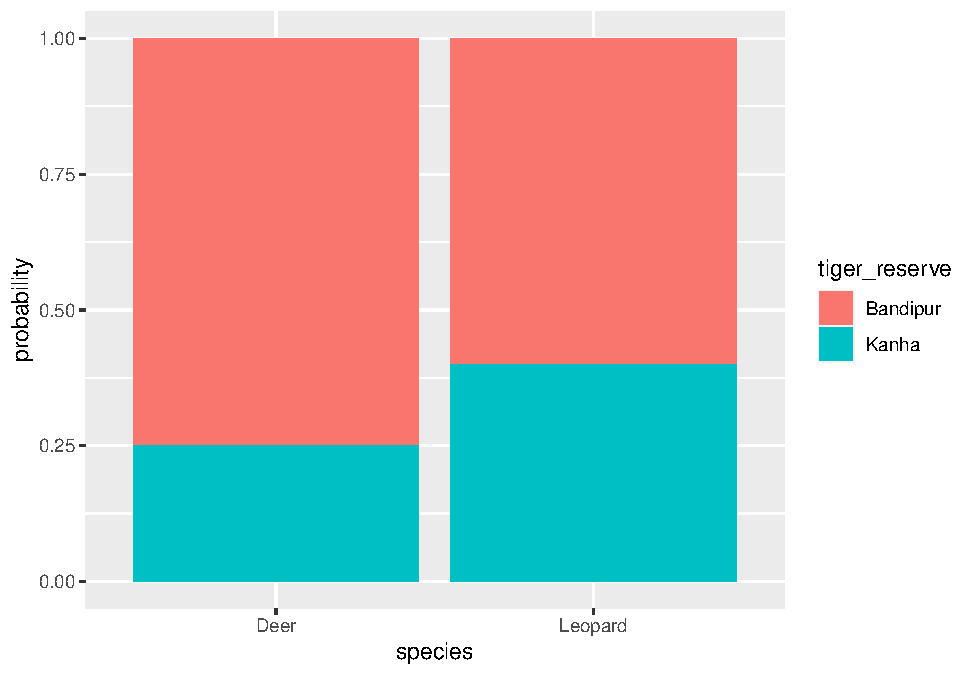
\includegraphics{_main_files/figure-latex/unnamed-chunk-73-1.pdf}
\caption{\label{fig:unnamed-chunk-73}Probability}
\end{figure}

  \bibliography{book.bib,packages.bib}

\end{document}
